\documentclass[12pt,a4paper,fleqn, onesside]{report}
%
\usepackage[T1]{fontenc}
\usepackage{amsmath, amssymb, amsthm}
\usepackage[danish,english]{babel}

\usepackage[ansinew]{inputenc}
%\usepackage[utf8]{inputenc} %Der skal anvendes utf8
\usepackage{epsfig}
\usepackage{graphicx}
\usepackage[]{mcode}
\usepackage{lmodern}
\usepackage{float}
\usepackage{setspace}
\usepackage{lscape}
\usepackage{hyperref}
\usepackage{cleveref}
\crefname{equation}{}{equations}
\crefname{figure}{figure}{figures}
\usepackage{tabu}
\usepackage{graphicx}
\usepackage{caption}
\usepackage{multirow}
\usepackage{spverbatim}
\usepackage{dirtytalk}
\usepackage{gensymb}
\usepackage{pdfpages}
\usepackage{mathpazo}
\usepackage{algpseudocode}
\usepackage{bm}
\usepackage[official]{eurosym}
%\usepackage{subfig}
\usepackage{subfigure}
\usepackage{mathptmx}
\onehalfspacing

\usepackage[top=25mm, left=30mm, right=30mm,bottom=25mm,headsep=10mm, footskip=12mm]{geometry}
%
\usepackage{fancyhdr}
\pagestyle{fancyplain}
\lhead[\thepage]{}

\begin{document}

% PAGE DE TITRE
\begin{titlepage}
\begin{center}
\vspace{4cm}
\Huge{\sc 30330 Image Analysis with Microcomputer}\\
\vspace{0.8cm}
\large{\sc Project report\\}
\vspace{1.2cm}
%\Huge {\sc Exam Report}\\
%\vspace{2cm}
\normalsize{by}\\
\vspace{1.2cm}
{\sc
\large Katleen Blanchet s150798  \\ 
Titouan Boulmier s150810\\
}
%\o{}
\vspace{2cm}
\begin{center}

\includegraphics[scale=2.2]{dtulogo2.jpg}
\end{center} 
\vspace{3.1cm}
\normalsize{\today}\\
\vspace{1.37cm}
\includegraphics[scale=0.7]{dtulogo.jpg}\\
\vspace{0.2cm}
\normalsize{Technical University of Denmark \\ Department of Electrical Engineering \\
}
\end{center}
\end{titlepage}
%\newpage
\thispagestyle{empty}
\selectlanguage{english}

\pagebreak
\pagenumbering{Roman}
\setcounter{page}{1}
\setcounter{tocdepth}{4}
\setcounter{secnumdepth}{4} 
\def\chaptername{Part}

\section*{Abstract}
In order to solve the overpopulation issue, scientists are studying Mars features to make it habitable. In this context, a system capable of stabilizing, in real time, the rover arm in front of a Martian rock to allow researchers to study it could be helpful. This project intends to design such a system, through the realization of a depth mapping of the rock thanks to the structured light technique. First, a scene analysis is carried out to determine the camera and the needed aperture to get enough light and to choose an artificial light source capable of outshining the sunlight. To detect the beam spots projected as a unicolor grid by the green LED selected as additional light source, a color detection algorithm is performed in C/C++ with OpenCV, as well as a centroiding algorithm which takes into account the intensity of the pixels belonging to the points. Then, based on the triangulation principle, the distance camera-target is derived and implemented.

The system is verified, with an alternative equipment due to lack of time, through two indoor experiments with one laser beam point and a line of dots. The results are quite promising, since the errors between the calculated distance and the real one could be reduced with an improvement of the calibration and of the color detection. The real time computation is validated. An outdoor experiment has also confirmed that the artificial light source should be capable of outshining the sun on the Red Planet. Nevertheless, extra work is required to implement the real system and the use of patterns, other than a unicolor grid which cannot prevent patterns disorders, could permit to get a more accurate 3D map.
\newpage

\section*{Acknowledgments}
We would like to express our gratitude to our supervisor Prof. Alessandro S. Massaro for his advices throughout the duration of the project. 
\bigbreak
We would also like to thank Prof. John Leif J�rgensen for his availability when we had additional questions.
\bigbreak
Beside them, we thank the associate professors to the course who taught us the knowledge needed to carry out this project.
\newpage

% SOMMAIRE
\tableofcontents
\newpage
\pagenumbering{arabic}

% Intro
\section*{Introduction}
\addcontentsline{toc}{part}{Introduction}
\subsection*{Context}
\addcontentsline{toc}{subsection}{Context}
The research of habitable planet is one of the major concerns of human beings. Indeed, this discovery, in addition to give hope of locating another species, would bring solutions to overpopulation. According to scientists, the main criterion for life is water. Since the properties of celestial bodies are disparate, a habitable zone was defined, considering that water can only exist at a specific range of temperature. If the temperature of the planet is too low, the water will freeze and conversely, it will evaporate if the temperature is too warm. The habitable zone is not fixed; it moves with the evolution of the sun. Mars is thought to have belonged to the zone once, due to its most hospitable climate after Earth. For a matter of fact, NASA's Mars Reconnaissance Orbiter has recently provided a strong evidence of water currently flowing on the Red Planet. It may then be possible to live on Mars and that is the aim of Mars one project: send a colony over there. The terraforming, which would change characteristics of Mars to make it suitable for humans, is also worth considering before colonization. In order to do so, scientists need to learn more about the features of the planet. Orbiters and rovers are already scanning mars surface and soil. Nevertheless, they lack the depth information, only equipped of Two Dimensional (2D) cameras. Their three dimensional (3D) scans have permitted to acquire it and to print a Martian meteorite on Earth in 2014. This information is useful for a better understanding of the rocks properties but that is not enough. Some missing data have delayed the 3D print. It could be interesting to provide to scientists a real time 3D map of a selected rock. It would be easier to study stones but the map could also help the robot to stabilize. With wind and an uneven ground, the rover is liable to move. The pattern recognition of a rock would be more robust by adding a 3D map. Samples could be collected being sure that the robot has taken the right piece. 

Furthermore, the 3D map could have several other applications. The features of the Martian soil acquired by the orbiting satellites are not exhaustive and lack of accuracy. Thus, applied to the area in front of the robot, the 3D map could detect new obstacles and update in real time the available map to distinguish modifications of the ground. It could also permit spacecrafts to determine a flat area to land in real time by analyzing the surface of the planet from space and during the descent. Moreover, the 3D map has other applications in completely different fields. Indeed, this technical can found, as example, in video games with environment recordings for real time augmented reality gaming, in medicine with skin surface measurement or skin roughness measurement, in cosmetic with wrinkle measurement and also in industry with 3D-automated optical inspection, volume measurement or Classification of grinding materials and tools.

However, the 3D mapping is not much used and is still improving. In this context, designing a system capable of carrying out a 3D map of a Martian rock would be profitable for future research. This is the purpose of this project, undertaken during the Image Analysis with Microcomputer course, under the supervision of Alessandro Massaro. Combining image and scene analysis, programming and robotics seems relevant for learning to work as an engineer.

This report is intended to our fellow students. The first part will bring additional knowledge required to understand the next developments. The design of the system is described in the next section, followed by its verification. To end, future work is addressed.
\subsection*{Problem formulation}
\addcontentsline{toc}{subsection}{Problem formulation}
\begin{figure}[H]
  \centering
  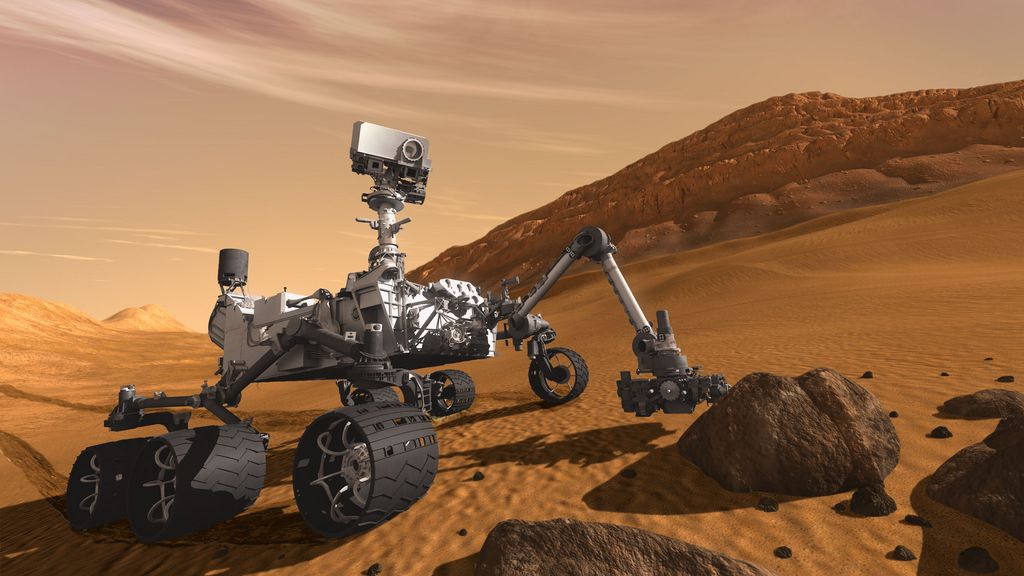
\includegraphics[scale=0.5]{fig/marsRover.jpg}
  \caption{Curiosity Rover with an embedded camera on a arm \cite{nasa}}
  \label{fig:CuriosityRover}
\end{figure}

In this report, we assume that we would like to send a rover on Mars, capable of communicating with Earth. Self-powered by solar panels, it will land at latitude 50� where it could get enough sunlight to recharge its lithium batteries. It is provided with an arm whose hand is replaced with a camera (see figure \ref{fig:CuriosityRover}). The latter will be used by scientists to observe relevant rocks to study. In order to accomplish this mission, once a stone is designed, the camera must be able to keep it in focus, despite the wind, the movement of the robot or any other perturbation. This implies a real time image analysis to be able to rectify the position of the camera. As a robust method is needed to maintain the stone in front of the arm, the correspondence problem is achieved by carrying out a 3D map of the surface. A luminous source should then be added to the rover to be projected on the surface containing the rock and detected by the camera.

This luminous source must be powerful enough to outshine the sunlight during the day, notwithstanding that the energy needed to make it work has to be negligible compared to the amount provided to the rover. Moreover, the characteristics of the camera need to be perfectly adapted to Mars, as once the rover has landed on the red planet, it would be impossible to adjust it. 

Will it be feasible to design such an embedded system, composed of a camera, a luminous source and algorithms, capable of keeping a rock in focus thanks to a 3D map, for an application on Mars soil? 

\subsection*{Problem delimitation}
\addcontentsline{toc}{subsection}{Problem delimitation}
In order to design the rover's camera which will be used to study rocks and to implement a robust algorithm to carry out a 3D map of the rock's surface, different characteristics of Mars and of the target need to be specified. However, as all of them cannot be taken into account, some simplifications and choices will be assumed.

\paragraph*{Mars delimitation}
~\\
Plenty of missions on Mars have been realized and a great deal of data has already been gathered. Nevertheless, even if some of them will be used to designed our system, others will be simplified or even ignored.
The first simplification concern the atmosphere of Mars. Indeed, even if its composition is now well know, it will be assumed that the dirt on the surface Mars plus the different layers of the atmosphere absorb, or scatter, 10\% of the solar energy. Moreover, the influence on the image acquisition that the dirt between the target and the camera could have will not be taken into account.
The second reduction cover the temperature. Indeed, even if it can reach -143\textdegree C during winter, 27\textdegree C during summer and have around 60\textdegree C variations between daytime and nighttime\cite{wiki:temperature}, we will assume that the CCD sensor works well all the time.

\paragraph*{Target delimitation}
~\\
Regarding the target, that is to say the part of the rock being studied, it is supposed to :
\begin{itemize}
\item be vertical;
\item not exceed 2*2 meters
\item have an area between 0.1 and 1 square meters;
\item have a relief less than  meters.
\end{itemize}

\paragraph*{Camera delimitation}
~\\
Then, regarding the camera which is designed during this study, it is presumed to :
\begin{itemize}
\item be between one and two meters far from the target;
\item be right in front of the target, that is to say that the angle between the normal of the target's surface and the focal axis of the camera is 0\textdegree;
\item be able to capture the image of a target of 2 meters height maximum.
\end{itemize}

The different characteristics of target and the camera are represented figure \ref{fig:schema system}


\begin{figure}[h]
  %\centering
  \centerline{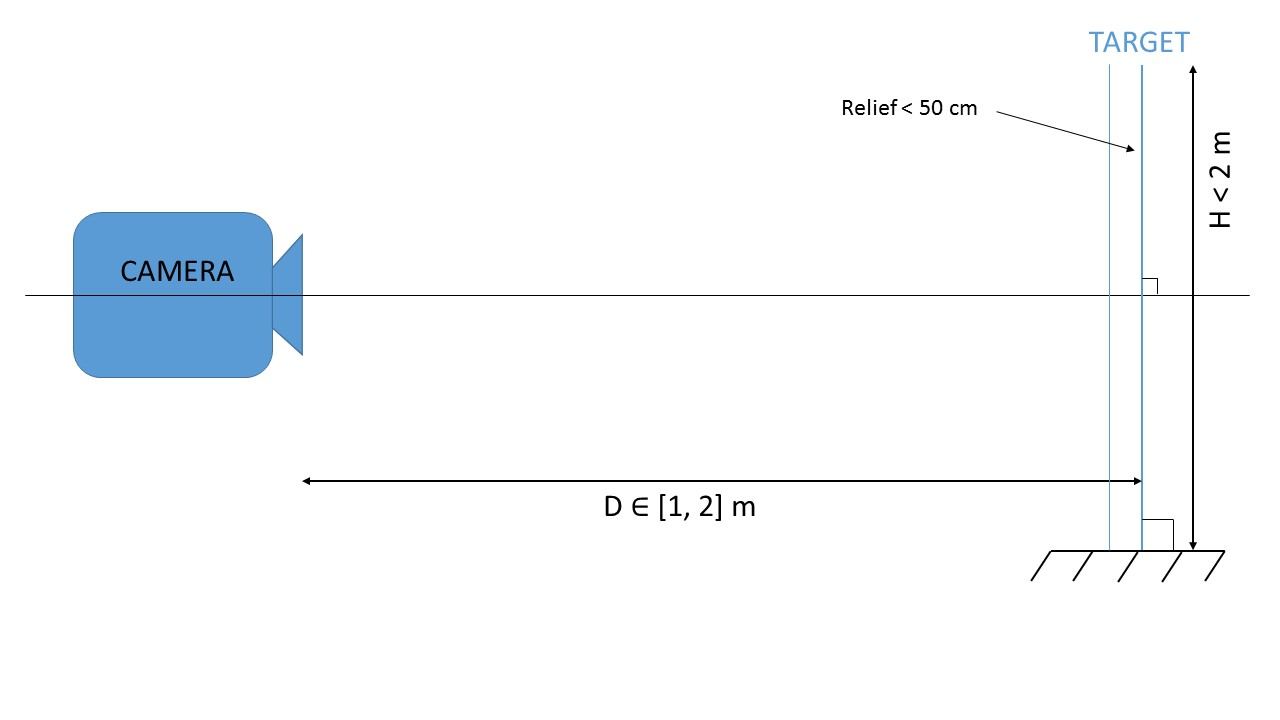
\includegraphics[scale=0.4]{fig/schemaSystem.jpg}}
  \caption{Schema of the scene}
  \label{fig:schema system}
\end{figure}



%theory section
\chapter{Theory Section}
\section{Mars Features}
Mars, the fourth planet from the Sun (1.3814 to 1.6660 AU) is the second smallest planet of the the Solar System (its radius is 3389.5 km). Known as the ``Red Planet'' because of the amount of iron oxide on its surface, it has an orbital period of 668.6 sols (Mars' solar day), that is to say 687 days, with an average day length of 24h37m.
\subsection{Atmosphere of Mars}
Because of its thin atmosphere, Mars has surface features which present analogies with both Moon, through the impact craters, and Earth, with volcanoes, deserts, polar ice caps. It is mainly composed of carbon dioxide $CO_2$ (96,0 \% $\pm$ 0,7 \%), argon $Ar$ (1,93 \% $\pm$ 0,01 \%) and oxygen
$O_2$ (0,145 \% $\pm$ 0,009 \%). As the gravity of Mars is low, the height of the atmosphere is 11 km, more than one and a half times higher than the Earth's one (7 km). Moreover, due to this low gravity, the wind can disrupt a rover easier than on Earth and a large amount of suspended dust is perpetually present at the surface.

Regarding the dust, of which the particles have a mean diameter of $1,5 \micro m$, is continually injected into the atmosphere by wind or dust devils (a 12 km high one can be seen 12 Figure \ref{fig:poussiere}). Such eddies are far from anecdotal because they bring dust to significant volumes of the atmosphere. Even if the amount of dust is never very massive, it can be lifted by winds slower than 2 $m/s$ and maintained indefinitely by wind of only 0,8 $m/s$.

\begin{figure}[h]
  \centerline{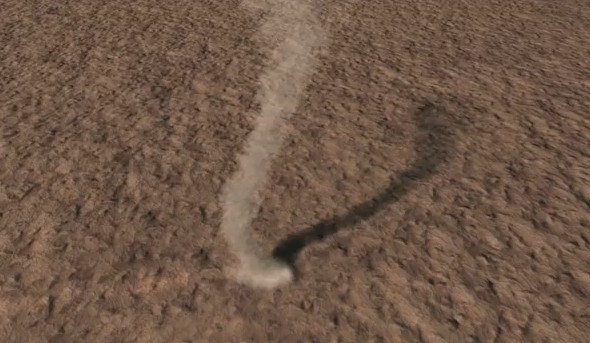
\includegraphics[scale=0.6]{fig/poussiere.jpg}}
  \caption{Dust Devil. Mars Reconnaissance Orbiter, made by HiRISE on Feb. 16, 2012}
  \label{fig:poussiere}
\end{figure}

Moreover, regarding the wind on Mars, in low altitudes, the Hadley circulation\footnote{movement on a planetary level of the layers of gases surrounding the planet} dominate and is almost the same process which, on Earth, generate the Trade winds. In high altitudes, a battery of areas of high and low pressure, named baroclinic pressure waves\footnote{In meteorology a baroclinic atmosphere is one for which the density depends on both the temperature and the pressure}, dominates the weather. The Mars wind lift a large amount of dust and can even trigger huge dust storms which can affect the while atmosphere (see Figure \ref{fig:storm}). Cyclonic storms can also appears on Mars. Indeed, cyclones similar to the ones of Earth tend to create during summer in the northern hemisphere but only in high latitudes.

\begin{figure}[h]
  \centerline{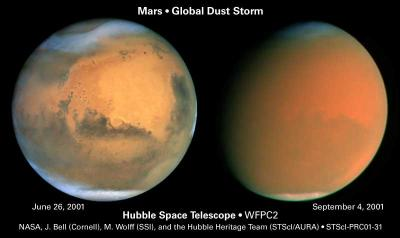
\includegraphics[scale=0.9]{fig/storm.jpg}}
  \caption{Two views of Mars with spatial telescope Hubble before and after the big dust storm in 2001}
  \label{fig:storm}
\end{figure}
\subsection{Climate of Mars}
\label{climate}
Because of its distance to the Sun bigger than the one of Earth, Mars receives less solar energy \ref{Irradiance}. Additionally, as its atmosphere is thinner, there is only a negligible greenhouse effect, and hence the average temperature is around -63\textdegree C on the surface of Mars with wide variations between daylight and night. \\
Then, the obliquity of Mars is close to the one of Earth (respectively 25,19\textdegree and 23,44\textdegree) but the eccentricity of Mars is bigger (0,09332 against 0,01671 for Earth) which means that, if Mars has similar seasons to Earth, they have different intensity and duration during the martian year. Thus, the northern hemisphere has seasons less pronounced than the southern hemisphere because its aphelion is at the end of spring and its perihelion at the end of autumn. Thus, there are short and soft winters and long and fresh summers in the northern hemisphere. On the opposite, the southern hemisphere has very pronounced seasons with long and cold winters and short and warmer summers than in the northern hemisphere. That is why there are higher temperature differences in the south.
\subsection{Albedo}
\label{albedo}
Mars surface is covered by sand and volcanic rocks. The first purpose of this project is to allow scientists to examine these rocks through the camera. To achieve it, it is needed to know their characteristics, especially their albedo. As a reminder, the albedo is the fraction of incident light which is reflected from a surface. We can assume that the power reflection of Martian rocks is the same than on Earth. Then, to cover a wild range of rocks, the albedos of a black and of a white stone would be considered. Charcoal, as a dark rock, is a powerful absorber of the sun radiation, with an albedo around 0.05. On the contrary, chalks are poor absorbers and their albedo reach 0.45 according to \cite{albedo}. In the following parts of the report, it will be taken for granted that Martian rocks have an albedo between 5 and 45\%.
\section{State of Art of the Depth Mapping}
Traditional cameras only take 2D pictures, with horizontal and vertical information. To reproduce the human vision useful in various applications such as the stabilization of a Martian rover arm in front of a rock to be analysed, it is often needed to add the depth data to get 3D coordinates of each pixel of the images. The depth mapping, also called 3D surface measurement or 3D imaging techniques etc, is carried out by two non-contact major methods as specified by \cite{sansoni2009state}: \say{projecting (in the active form) or acquiring (in the passive form) electromagnetic energy onto/from an object followed by recording the transmitted or reflected energy}. They can be divided into two categories, the non-optical and optical sensing. The first one generally uses acoustic and electromagnetic sensors to determine the distance from the system to the object, by assessing the duration of a round trip of a pulse. In the latter the light permits to get the depth. We will focus on this last technique as it will be more convenient to achieve it on Mars. Active optical sensing uses an additional light source where as passive optical sensing works only with the irradiance reaching the scene and the radiance of the object. 

\subsection{Principal Techniques Based on Image Analysis}
We will address only methods using image analysis as this is the purpose of the course.
Stereo vision and Photogrammetry systems are passive. The principle of the first is based on the utilisation of two or more cameras to record the scene. The reconstruction of the 3D is carried out by solving a correspondence problem with the identification of patterns in two or several images. The photogrammetry method calculates the depth by taking pictures from different points of view of a scene, through a camera preliminary calibrated. Both techniques demand a high computing power. Thus they are dismissed since the Rover cannot provide too much power to the embedded processor. 

In active optical sensing, laser triangulators and structured light can be distinguished. They share the same approach: a beam or a pattern is projected through a laser source towards the object and its position on the image acquired by the camera is measured. Then, the distance from the camera to the object (the depth) is found by applying a triangulation technique. The difference between the two methods is that it is needed to scan the whole object for the laser triangulators one. Indeed, only a beam or a laser strip reaches it at once. The experiment has to be repeated several times to have an exhaustive 3D map. Regarding the structured light approach, unique patterns are projected simultaneously which allows to obtain the depth data at once if the object is small but in any case, it reduces a lot the number of acquisitions compared to the laser triangulators. According to \cite{tuto}, the patterns can be in 3D but they are rare. 2D patterns are the most common and easier to implement. Depending on the scene motion, the structured light method can be classified into multi-shot and single-shot. If the scene is moving, the acquisition time must be short and thus, one picture should be enough to get the desired information. On the other hand, if no constraint is given, several pictures can be taken and a pattern adapted to sequential can be selected. In our case, the scene does not move but the robot arm could move and thus needs to be stabilized. That is why only single-shot structured light will be considered.

In the future part of the report, the implementation and experiments will be performed through laser triangulators techniques and structured light with a unicolor grid as a pattern. They are easier to set up but will only give us a partial depth map. To obtain a complete 3D map in a single shot, more complex patterns should be applied to the martian rock. Some methods that could be carried out then are described below. 
\subsection{M-array Pattern Projection Method \cite{morita1988reconstruction}}

The binary M-array pattern projection method consists in projecting dark and light dots. The color of each dot represents a 0 (dark) or 1 (light) of the M-array pattern. The spatial coordinates of each dot matched with a projected one of the pattern can be determined by triangulation. However, pattern disorders occur often in the observed pattern and some dots cannot be matched. One of the asset of this method is the detection and correction of pattern disorders.

\subsubsection{Pattern Disorders}
\label{PatternDisorders}
According to \cite{morita1988reconstruction}, there are three different types of pattern disorder.
\begin{itemize}
\item Deficiency of dots. If there are several objects in the scene, an object may obstruct the pattern. On the Figure \ref{fig:disorder1}, the first, second and third dots are not visible by the camera.
\item Displacement due to Difference in Depth : in comparison to the initial pattern projected, the dots may shift because of the depth of each object. On the Figure \ref{fig:disorder1}, the dots 4 to 6 on the object 2 have shifted to the left compared with the dots of object 1.
\item Permutation of dots : if an object is in front of another, the order of dots may change. On the Figure \ref{fig:disorder1}, the dot 3 has changed of order and is the fourth one from the point of view of the camera.
\end{itemize}

\begin{figure}[h]
  %\centering
  \centerline{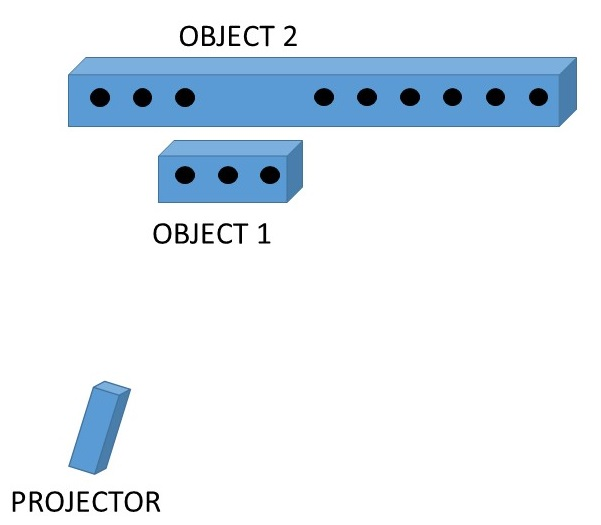
\includegraphics[scale=0.6]{fig/disorder1.jpg}}
  \caption{Pattern Disorders}
  \label{fig:disorder1}
\end{figure}






\subsubsection{Correction of Pattern Disorders}
There are four steps in the matching of the observed dots with those of the pattern and the correction of the pattern disorders.





\paragraph*{Temporary Array}
~~\\
The image recorded is analyzed line per line of dots and a 2-D array which contains the numbers of the observed dots is created. The array can be computed by these steps :
\begin{itemize}
\item Creation of the array (all the elements are set to zero).
\item Scan of the image to detect dots. Each time a dot is found, its value and position (center) are saved into 1-D arrays VALUE, X and Y.
\item The position of the dots are quantized using X and Y so that adjoining dots have consecutive quantized coordinates.
\item Insertion of the number of each dot into the array (the location into the array corresponds to the quantized coordinates).
\end{itemize}

This temporary array (T-array) may has some vacant places due to disorder pattern.

\paragraph*{Grow}
~~\\
Each element of the T-array gets an index (column number of the M-array). To do so, a window is defined and applied to the T-array and the M-array where the elements into the window of each array have the same value. The element into the window of the T-array can be indexed using the M-array and the two windows moved simultaneously by one column or row. This is repeated until a difference between the two windows is detected. New windows are then initialized elsewhere. The grow terminate when no window can be initialized to an area of the T-array where there is no index yet.


\paragraph*{Correction of Pattern Disorders}
~~\\
The detection step is is carried out during the growing and is explain below using an example. We use a 3$\times$4 window.
\begin{itemize}
\item step 1 : the region growing starts at (0',0') and (0,0) on the T-array and M-array (see Figure \ref{fig:detect} a).
\item step 2 : the window slides to the right until a difference between the two arrays is detected (see Figure \ref{fig:detect} b).
\item step 3 : In the T-array, the window is shifted to the right until the error is on the left side of the window. In the M-array, the window is moved until it matches with the one of the T-array (see Figure \ref{fig:detect} c).
\item step 4 : the windows now slides to the left and all the indices of the columns of the T-array are reset according to the two windows until another difference is detected.
\end{itemize}

\begin{figure}[h]
	\centering
	\hspace*{-2cm}
   \begin{minipage}[b]{0.50\linewidth}
      \centering 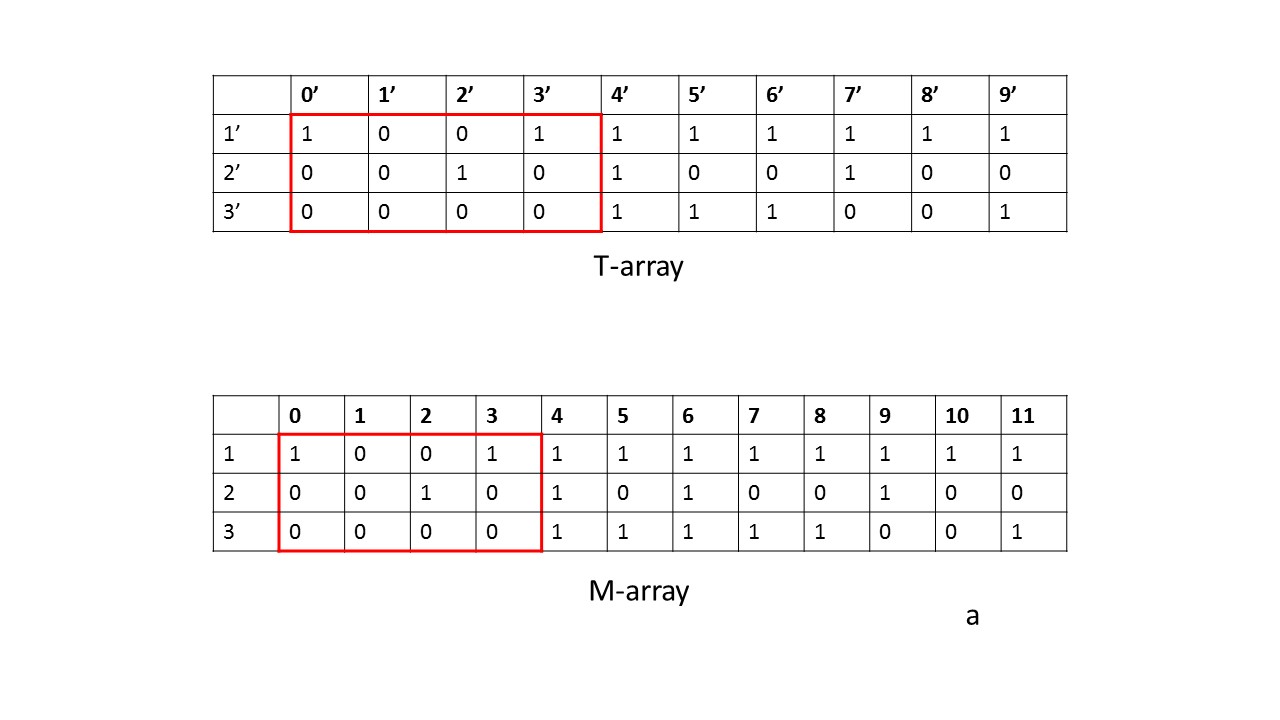
\includegraphics[scale=0.3]{fig/detect1.jpg}
      %\caption{\it Legend 1}
   \end{minipage}\hfill
   \begin{minipage}[b]{0.50\linewidth}   
      \centering 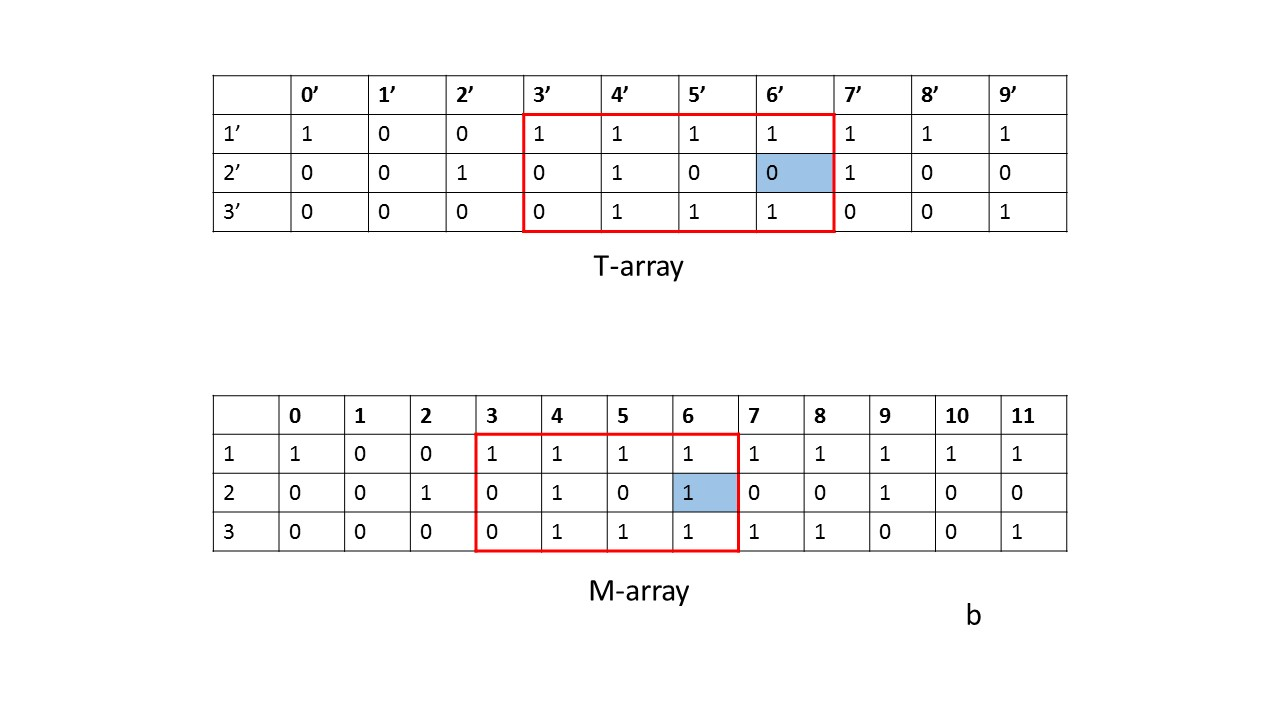
\includegraphics[scale=0.3]{fig/detect2.jpg}
      %\caption{Legend 2}
   \end{minipage}
	\hspace*{-2cm}
   \begin{minipage}[b]{0.50\linewidth}
      \centering 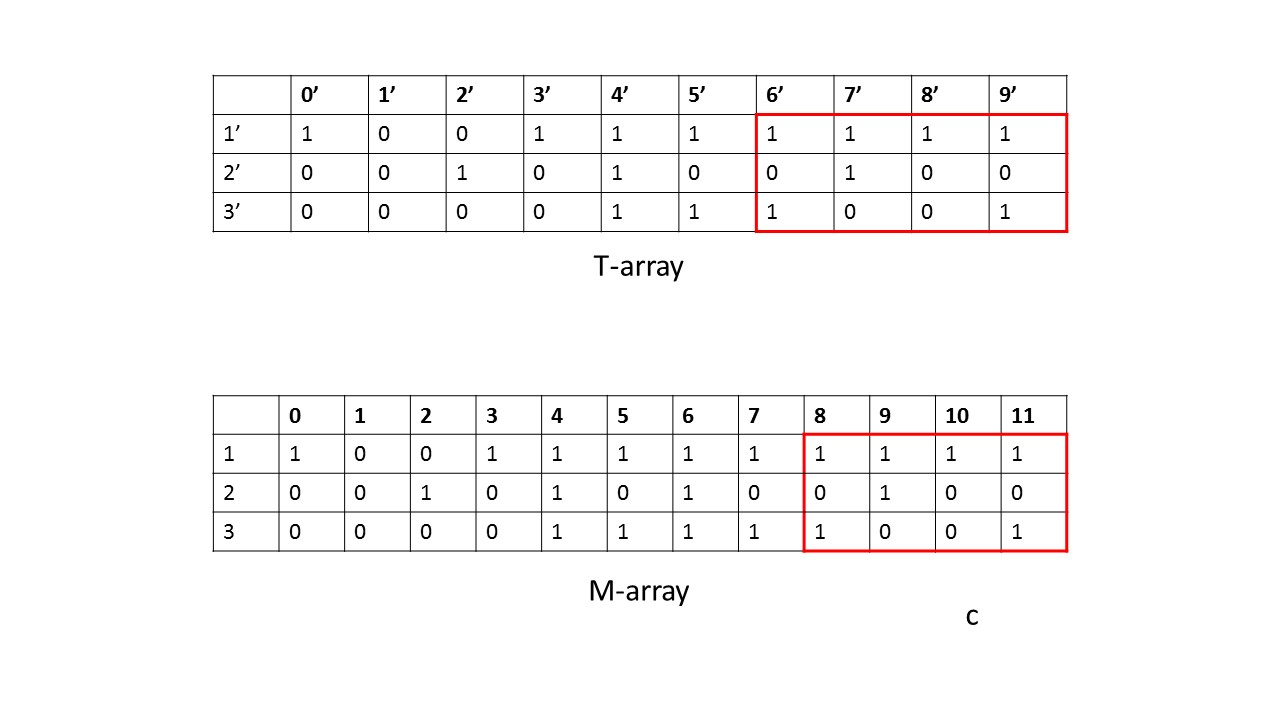
\includegraphics[scale=0.3]{fig/detect3.jpg}
      %\caption{Legend 3}
   \end{minipage}\hfill
   \begin{minipage}[b]{0.50\linewidth}   
      \centering 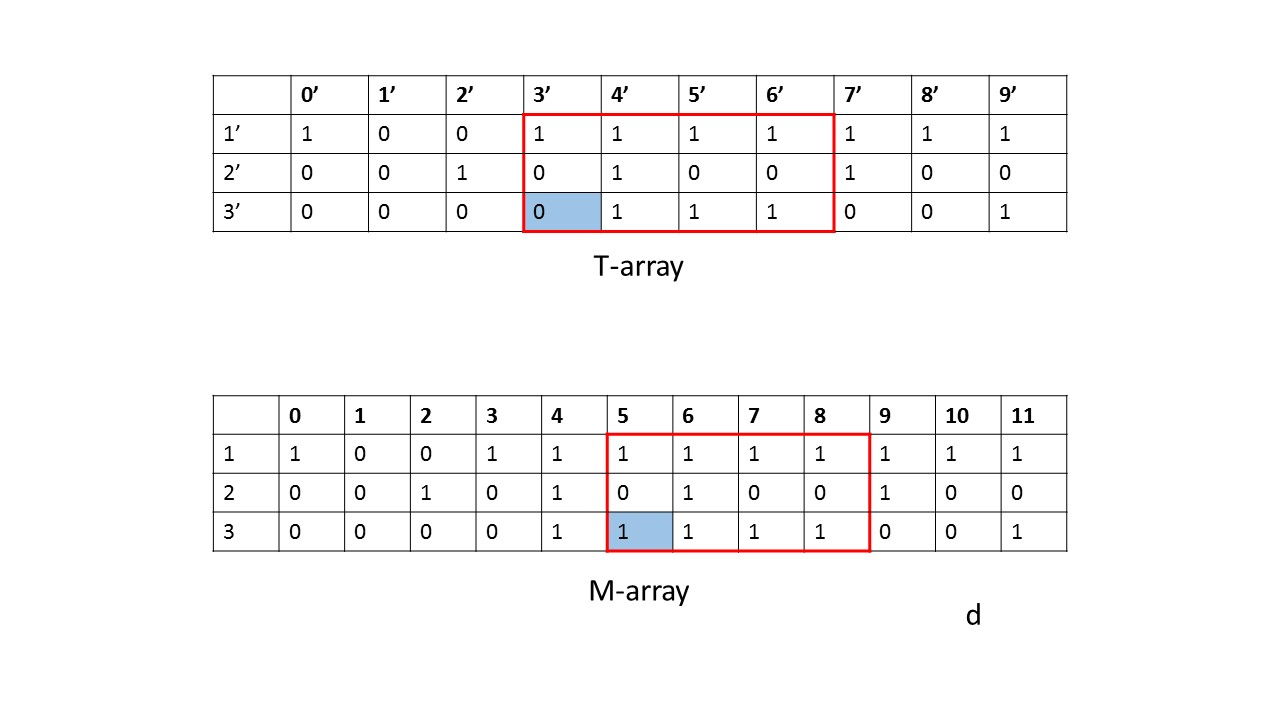
\includegraphics[scale=0.3]{fig/detect4.jpg}
     % \caption{Legend 4}
   \end{minipage}
	\caption{Detection of the disorders}
	\label{fig:detect}
\end{figure}


Then, as regions of the T-array extends because of the step 4, a new window can be initialized on the extended region and the growing starts again. At the end, except some array cells corresponding to dots lighted near the border of two objects, all the indices of the T-array have been determined.










\paragraph*{Detection of Pattern Disorders}
~~\\
Knowing that, in the T-array, the elements which still have no indices appear to be mostly alone or draw a chain, some rules permit to correct the index of these elements.

\begin{itemize}
\item if the element at the top and at the bot have the same index k, the current element has also this index k.
\item if the element at the left has the index k-1 and the one at the right k+1, then the current element has the index k.
\item the difference between the index of two horizontal neighbors corresponding to closer positions on the image is one.
\item if the indices of a consecutive vertical sequence are still undetermined, they get the index of the element at the top or bottom of the vertical.

\item if the indices of an consecutive horizontal sequence are still undetermined, they get the index such as it increases by one from index determined on the left to the on the right.
\begin{tabular}{|*{11}{c|}}
    \hline
     k-5  & k-4  & k-3  & \textcolor[rgb]{1,0,0}{k-2}  & \textcolor[rgb]{1,0,0}{k-1}  & \textcolor[rgb]{1,0,0}{k}  & \textcolor[rgb]{1,0,0}{k+1}  & k+2  & k+3  & k+4 & k+5 \\
    \hline
\end{tabular}
\end{itemize}

According to \cite{morita1988reconstruction}, the previous rules should correct the most of the errors of indexation and the cases where the error cannot be corrected are scarce.







\subsection{Grid Indexing}

The method of the binary M-array projection is based on the matching of a binary array, but other patterns can be used too to permit the matching of the projected and observed patterns. A non-exhaustive list of grid indexing is presented below.

\subsubsection{Mini-patterns Used as Code Words}

Instead of using a binary array, a technique can be using a array of words coded by patterns. Each pattern codes a word. As instance, on the figure \ref{fig:codeWords}, three words has been coded and permits to convert the projected pattern into a array of integers.


\begin{figure}[h]
  %\centering
  \centerline{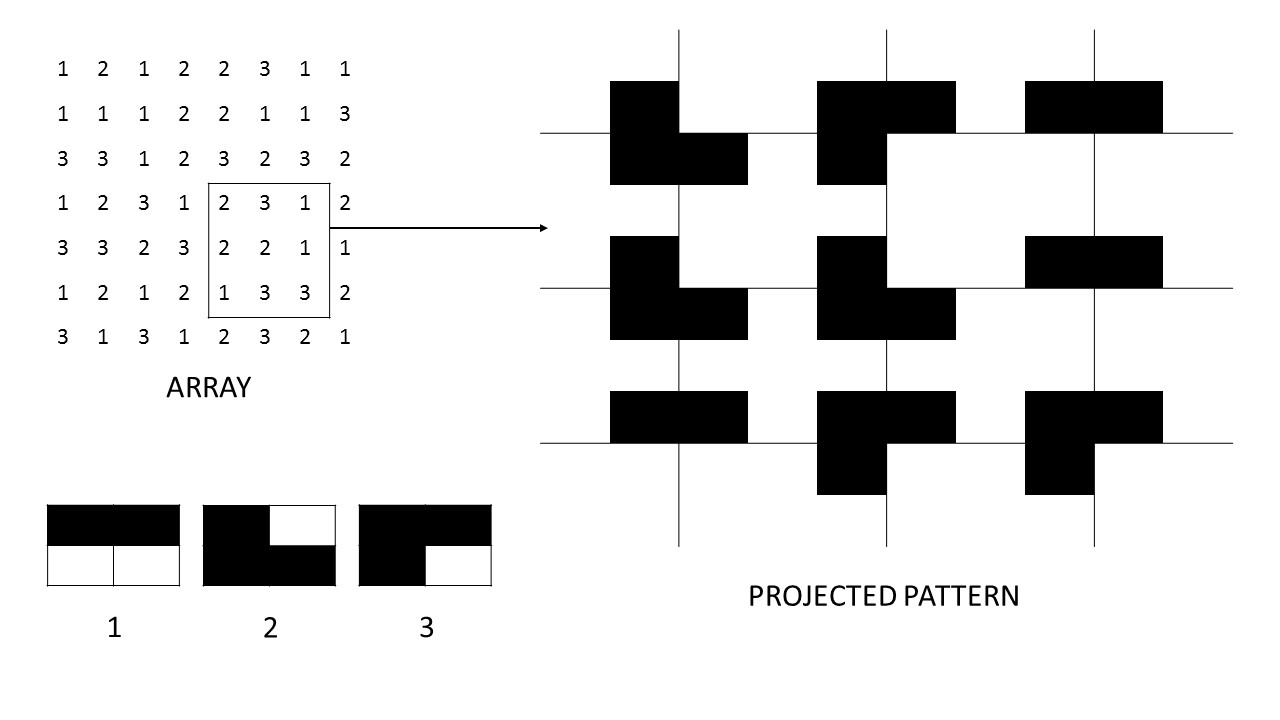
\includegraphics[scale=0.5]{fig/codeWords.jpg}}
  \caption{Mini-pattern used as code words}
  \label{fig:codeWords}
\end{figure}





\subsubsection{2D Array of Color-coded Dots}

Another technique is the 2D array of color-coded dots. The concept of this method is almost the same as the previous one but instead of using pattern to code a word, colors are used (see Figure \ref{fig:color-coded}).

\begin{figure}[h]
  %\centering
  \centerline{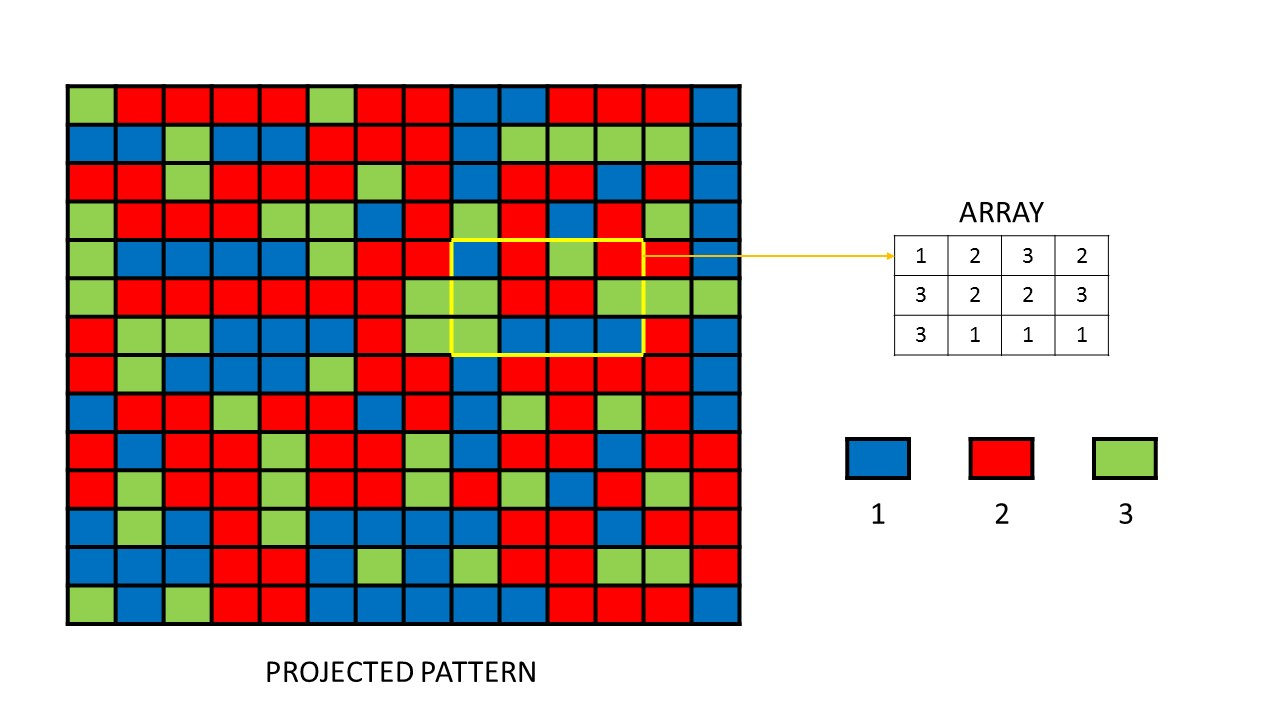
\includegraphics[scale=0.5]{fig/color-coded.jpg}}
  \caption{2D Array of Color-coded Dots}
  \label{fig:color-coded}
\end{figure}

\section{Image processing}
In the following part of this report, the color detection will be used to distinguish color light points projected by a luminous source on a Martian rocks from its background. In order to implement this color detection, the HSV color model needs to be defined, as well as some morphological operations. 

\subsection{HSV Color System}
HSV stands for Hue Saturation Value. It is a color system which allows the separation of the color components from the intensity, unlike RGB system. It is more intuitive to find a plain object by varying HSV parameters.

The Hue designates the color itself. As it can be seen on the figure \ref{fig:HSV}, the color is determined by an angle between 0\degree and 360\degree. Red corresponds to 0�, green to 120� and blue to 240�. OpenCV range is 0-180. Changing the Saturation will affect the intensity of the color. A low value indicates a dull color. The Value has an impact on the luminosity of the color. Decreasing this value makes the color darker. The S and V are varying between 0 and 1 but the OpenCV range is 0-255.

\begin{figure}[H]
  \centering
  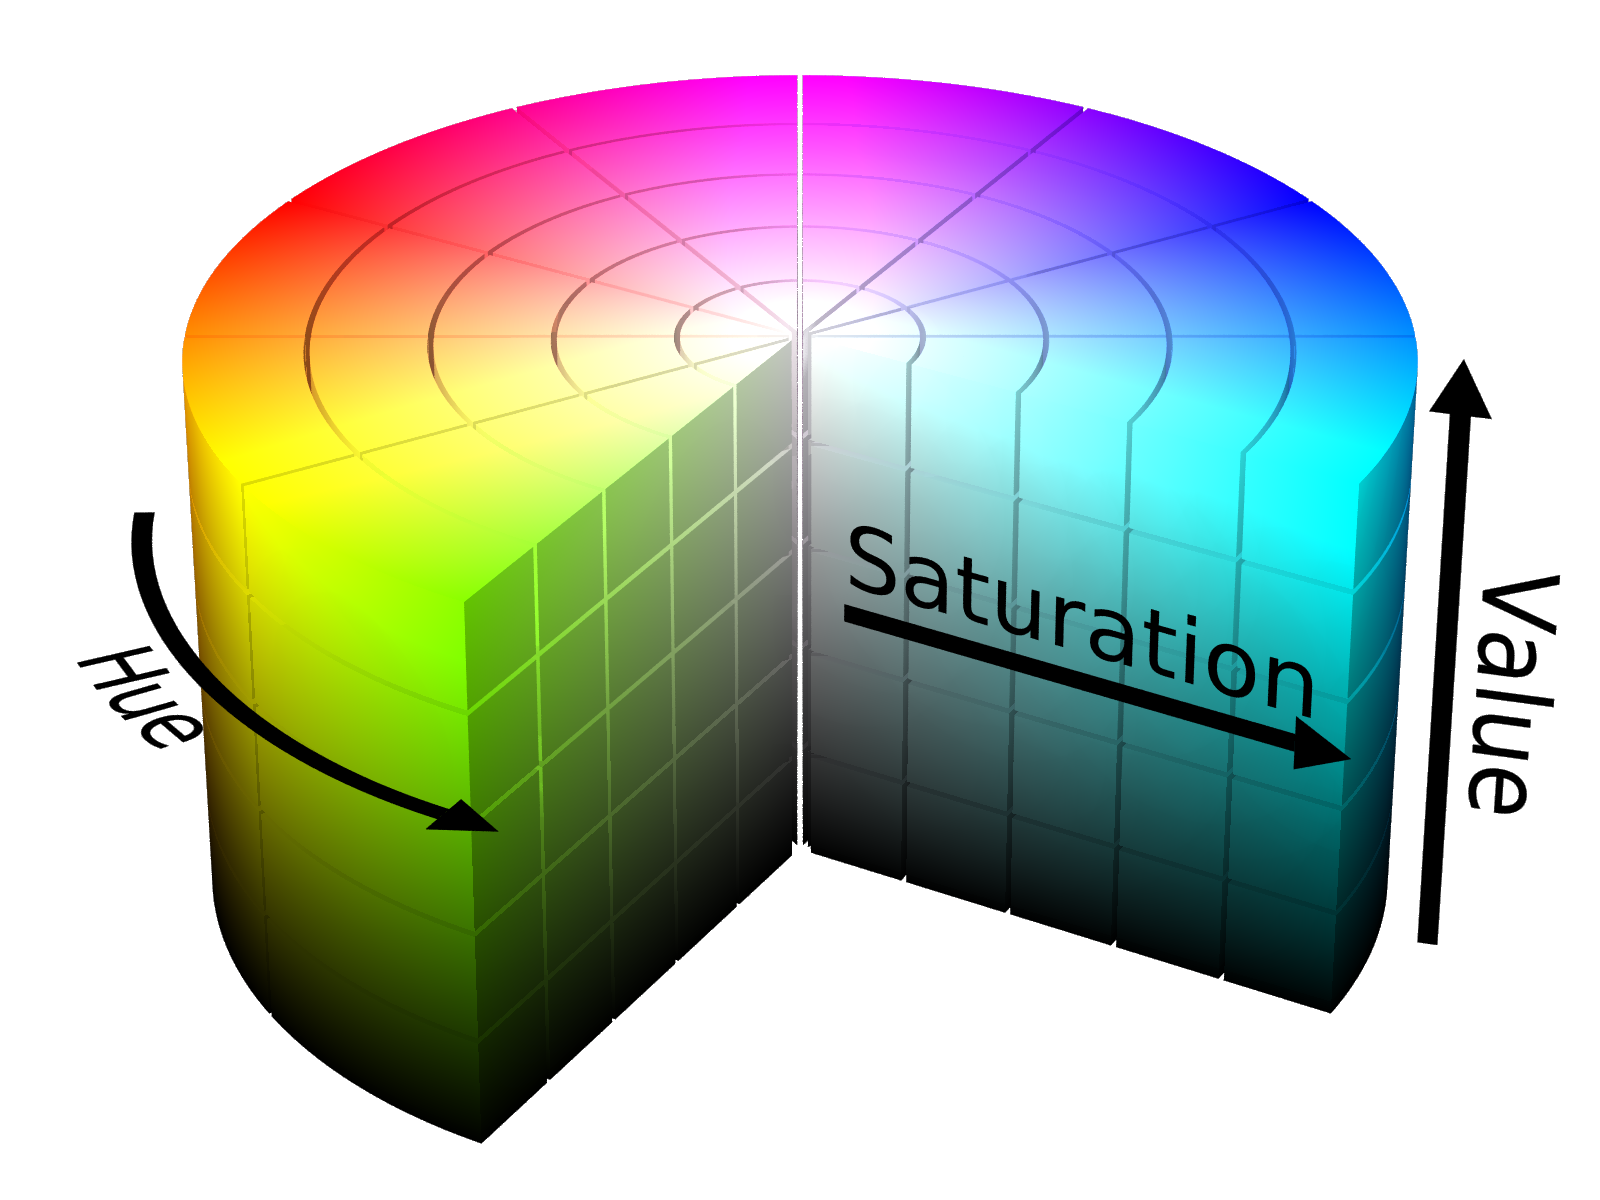
\includegraphics[scale=0.15]{fig/HSV.png}
  \caption{HSV diagram \cite{wiki:hsv}}
  \label{fig:HSV}
\end{figure}

\subsection{Morphological Operations \cite{bradski2008learning}}
The morphological operations on a binary image consists in applying a structuring element to each pixel of the object parts to reshape them. Two basic operations will be used later on and are explained here: the erosion and the dilation. Detailed diagram of the erosion and dilation can be found below (figures \ref{fig:erosion} and \ref{fig:dilation}). It should be noticed that for more legibility, the background is in white and the object in color. It will however be assumed that the pixels of the object have a value superior to the background.

\begin{figure}[h]
  \centering
  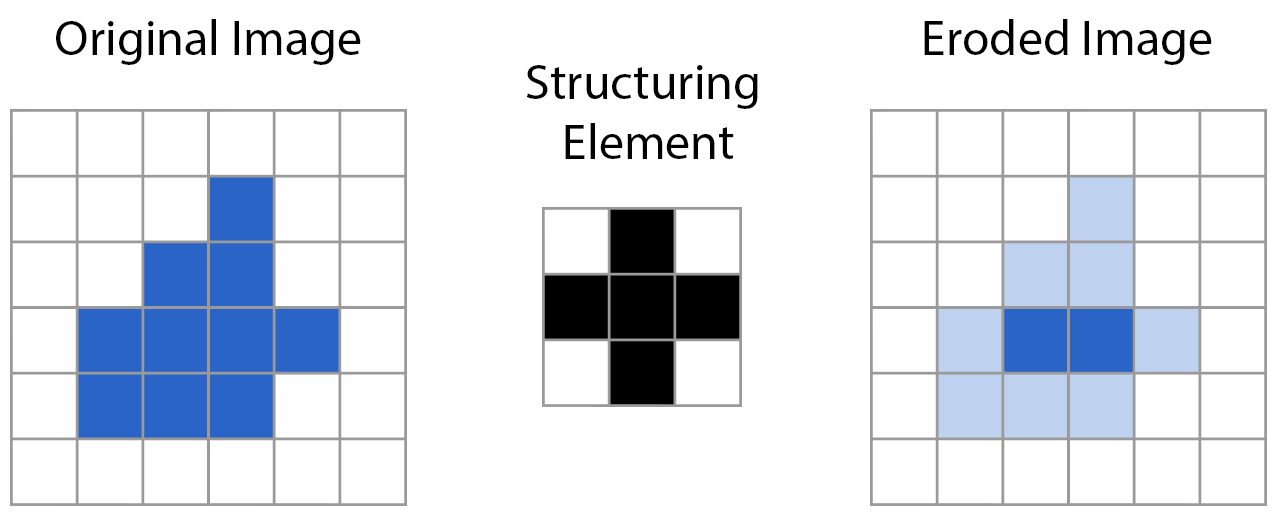
\includegraphics[scale=1]{fig/erosion.png}
  \caption{Erosion principle}
  \label{fig:erosion}
\end{figure}

\begin{figure}[h]
  \centering
  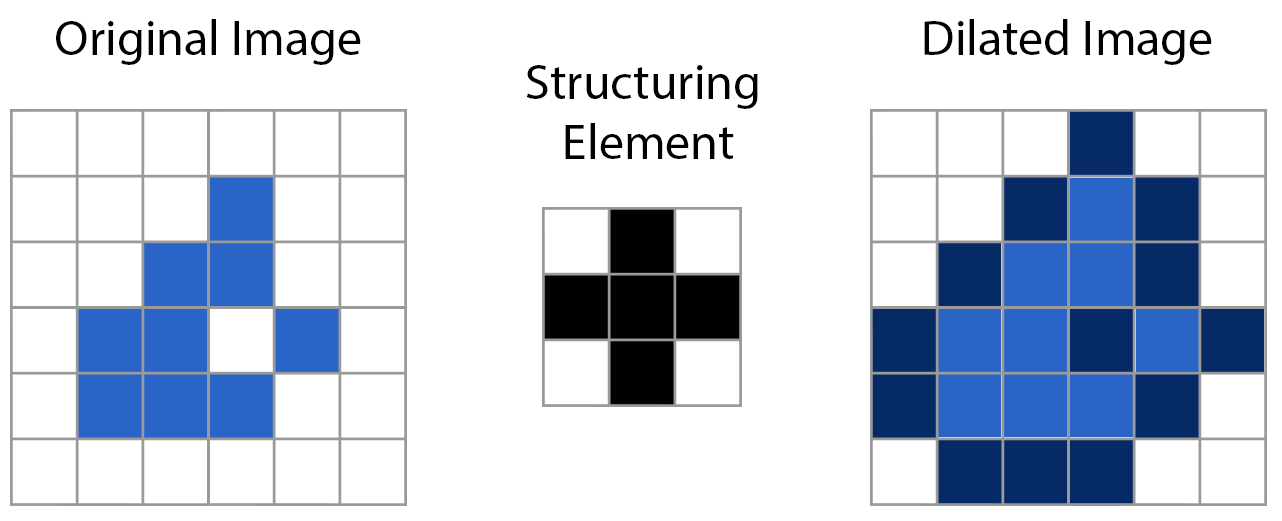
\includegraphics[scale=1]{fig/dilation.png}
  \caption{Dilation principle}
  \label{fig:dilation}
\end{figure}

\subsubsection{Erosion}
This transformation is similar to the logic gate AND. The structuring element or kernel is moved along the image and the minimal pixel value is set as the new value of the anchor point, in the figure, the center of the structuring element. This means that if all the points of the kernel are on an object (a white object on a black background), the anchor point will keep its value. On the contrary, if any element of the kernel is out of the object, the center point will become part of the background. The erosion is useful to separate two objects connected and to remove objects which are smaller than the size of the structuring element (noise). 

\subsubsection{Dilation}
The dilation is the opposite transformation of the erosion. It corresponds to the OR. If one element of the kernel is on the object (which is still assumed to have the maximal value for its pixel), the anchor point will be set to this value and thus be turned into a part of the object. This operation permits to fill holes in an object, to increase its size and to link objects which are closer than the size of the structuring element.

\subsubsection{Opening}
When combined, first by operating an erosion and then a dilation, the transformation is called an opening. The inverse operation is the closing. An opening could be convenient to separate luminous points which are connected and to then increase their size, lessen by the erosion to retrieve a shape similar to the original points.


%develepment section
\chapter{Development}
\section{Scene Analysis}
Into this section, the camera and the artificial light source are designed and the Signal/Noise ratio is calculated.
\subsection{Camera}
In order to design the camera and find its characteristics, a scene analysis have to be carried out. Our study is based on the MER (Mars Exploration Rover) cameras properties \cite{merengineeringcameras}.
To begin with, we choose an image sensor. 

\subsubsection{CCD}
\label{fig:CCD}
The Charge Coupled Device (CCD) is commonly more sensitive to light than its counterpart, the CMOS (Complementary Metal Oxide Semiconductor). Moreover, in the near infrared CCD appears to have a better response. Since Mars has a reddish color, it seems more accurate to select the CCD detector.

As scientists will need to discern the details of rocks, the resolution should be around the megapixel. Taking into account the cost, which will increase with the resolution, and the time of computation for an image with too many pixels, 1024 x 1024 seems to be an acceptable compromise.

Finally, the last element to consider is the pixel size. A trade-off have to be found between having a higher resolution (smaller pixels) and more sensitivity (larger pixels). All the camera of the MER mission were conceived with a pixel size of 12 x 12 $\mu m^2$ for a resolution of 1024 x 1024. It was decided to comply with that value.

For the next parts of this report, we will use the data sheet of the FTT1010M CCD image sensor (see Appendix \ref{CCDdatasheet}) as a basis for our calculations which will require CCD details.

\subsubsection{Field of View}
According to the book \cite{book}, the Field of View (FoV) \say{is the angle of the cone of directions encompassed by the scene that is being images}. This solid angle is needed to compute the focal length the camera should have.

\begin{figure}[h]
  \centering
  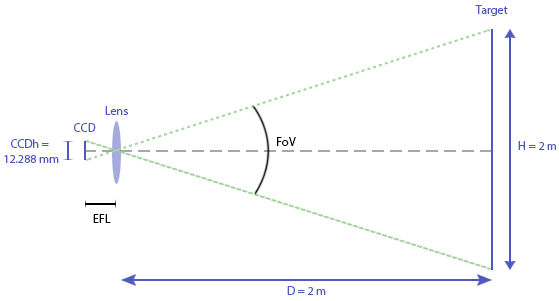
\includegraphics[scale=0.7]{fig/FOV.png}
  \caption{Field of View and Effective Focal Length}
  \label{fig:FOV}
\end{figure}

A simple relationship between the distance lens-target, the size of the target and the FoV can be deduced from the detailed diagram \ref{fig:FOV}: 
\begin{equation*}
tan( \frac{FoV}{2}) = \frac{1}{2} \times \frac{H}{D}
\end{equation*}
We derive and get
\begin{equation*}
 \frac{FoV}{2} = atan(\frac{1}{2} \times \frac{H}{D})
\end{equation*}

Numerically, with our problem delimitation, the Field of View is equal to $26.6\degree \times 26.6\degree$. 

\subsubsection{Focal Length}
\label{focalLength}
Thanks to the previous diagram, the Effective Focal Length (EFL) can also be determined: 
\begin{equation*}
EFL = \frac{1}{2} \times \frac{CCDh}{tan(\frac{FoV}{2})} = 12.29 \ mm
\end{equation*}
where $CCDh$ is the image section of the CCD according to the data sheet.\\

In order to get the real focal length, we choose $rf = 1 \ m$ for the distance of focus of the camera. 
\begin{equation*}
f = \frac{1}{\frac{1}{rf}+\frac{1}{EFL}} = 12.14 \ mm
\end{equation*}

\subsubsection{Aperture}
\label{aperture}
To determine the diameter of the aperture, several criteria have to be accounted for. If the diameter is too small, the sharpness of the image will decrease due to the diffraction effect. In fact, at large aperture, the diffracted light is negligible compared to the total amount of light entering the system. On the other hand, we should also consider the Depth of Field (FoV). We need to insure that it is big enough to allow us to see the whole target on the image. The relationship between the DoF and the diameter is inversely proportional. That means that if we increase the diameter, we will lessen it. The Diameter of Confusion (DoC), linked to the DoF is also a factor to take into consideration for the choice of the diameter. According to Wikipedia \cite{wiki:coc} It corresponds to \say{an optical spot caused by a cone of light rays from a lens not coming to a perfect focus when imaging a point source}. The smaller the DoC is, which corresponds to a better focus, the bigger is the DoF, and also the smaller is the diameter.

As the behaviour of the depth of field and of the diameter of confusion runs counter to the diffraction one, a trade-off has to be found. 

These formula are used to calculate the diameter of confusion and the diffraction spot:
\begin{equation*}
DoC = Dsr \cdot \frac{|r-rf|}{r} \cdot \frac{f}{rf - f}
\end{equation*}
where $Dsr$ is the diameter of the aperture
\begin{equation*}
DiffractionSpot = 2 \cdot EFL \cdot tan(1.22 \cdot \frac{lambda}{Dsr})
\end{equation*}
where $lambda$ is a wavelength of the sunlight\\

In the delimitations, it is assumed that the wavelengths of the sunlight belong to [400 800] nm. To settle on a diameter, the diameter of confusion and the diffraction spot were computed for diameters varying from 1 mm to 5 mm and wavelengths from 400 nm to 800 nm. The results are shown graphically in figure \ref{fig:DoCDifspot}. As the diameter of confusion cannot be bigger than the height of a pixel, the line corresponding to 12 $\mu m$ was also added to the graphic. In order to have the best trade-off, that is to say all the curves under 12 $\mu m$, we have chosen a effective lens entrance aperture $Dsr$ equal to $1.9 \ mm$, corresponding to $DoC = 0.0117 \ mm$. 

\begin{figure}[H]
  \centering
  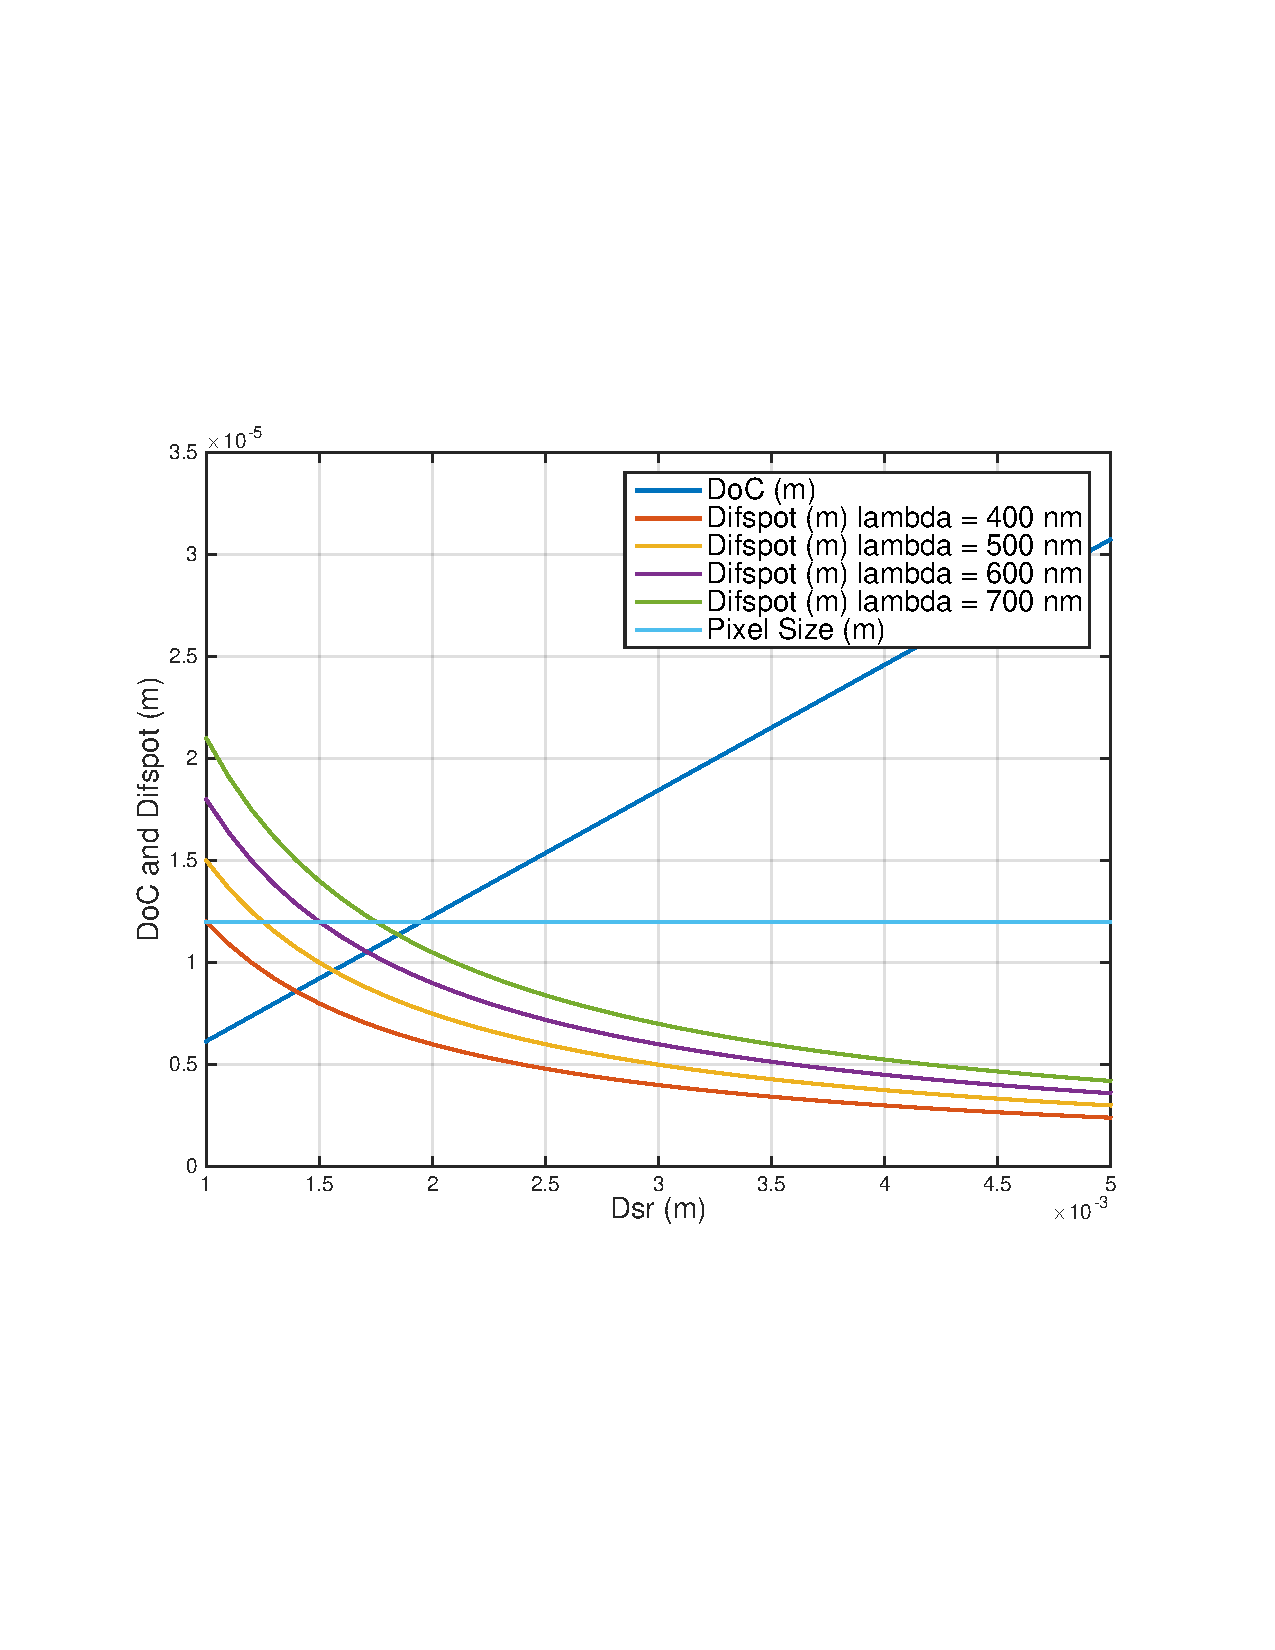
\includegraphics[trim=2cm 7cm 2cm 7cm, clip=true, totalheight=0.45\textheight, angle=0]{fig/DoCDifspot.pdf}
  \caption{Diameter of confusion and diffraction spots as a function of the diameter}
  \label{fig:DoCDifspot}
\end{figure}

Then, the depth of field can be deduced:
\begin{equation*}
DoF = \frac{2\frac{f}{Dsr}DoC(m+1)}{m^2 - (\frac{DoC}{Dsr})^2} = 1.33 \ m
\end{equation*}
That means that the roughness of the rock analysed cannot be more than $\frac{DoF}{2} =  66.5\ cm$ since we could not see the whole rock if not, and the 3D map will then be flawed.
\subsection{Artificial Light Source}
In order to carry out a 3D mapping of the target, the system needs a light source to project points which will be used by the 3D mapping algorithm. In this section, the source of light will be designed.

\subsubsection{Design of the Light Source}
~\\
First of all, the green has been chosen as color of the light source. Indeed, in order to detect easily the points projected on the target, a distinctive color should be used. As we can see figure \ref{fig:QeCCD}, the CCD selected for the camera has the best quantum efficiency for a wavelength around 510 $nm$, which means that the green is the color that is the best recorded by the camera. Secondly, as the surface on Mars is mainly orange, red and brown, this color should stand out.


\begin{figure}[h]
  %\centering
  \centerline{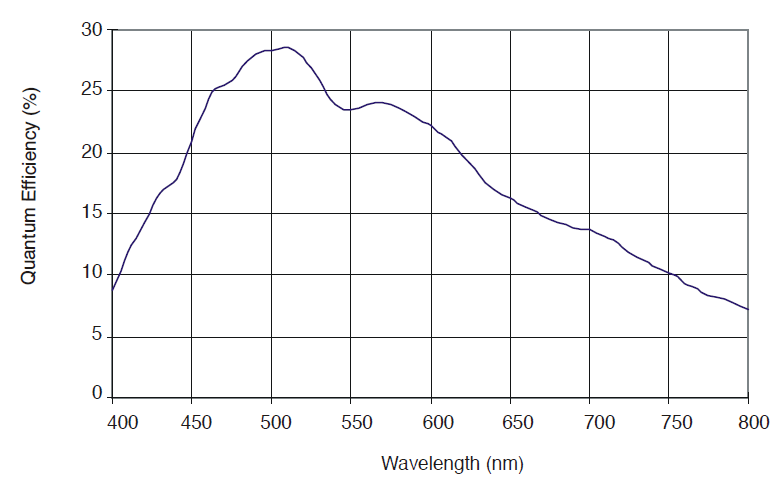
\includegraphics[scale=0.4]{fig/QeCCD.png}}
  \caption{Quantum efficiency versus wavelength of the CCD}
  \label{fig:QeCCD}
\end{figure}

Then, as only 300 $mW$ are available to aliment the light source and a lot of lightning energy is needed to outshine the sunlight, a LED has been chosen. Indeed, LEDs have great energy performances. The properties of the chosen LED can be seen in Annex \ref{LEDdatasheet}. Note that the use of a laser have been studied, but the energy cost would have been too expensive. Moreover, even if we cannot obtained a coherent light, as a laser do, with a LED, it is still feasible to obtain a monochromatic and directional light. Thus, we will assume that the LED can bring enough light (proof in part on Signal Noise Ratio\ref{light Power}).\
Then, as the 3D mapping algorithm needs a grid of points, the LED cannot be used in its present condition. Moreover, lot of light would be lost without an optic system. Thus, a system has been designed to concentrate the luminous beams of the LED and to transform the continuous light into a grid of point. The system uses a lens and a grid (Figure \ref{fig:LEDsystem}). 

\begin{figure}[h]
  %\centering
  \centerline{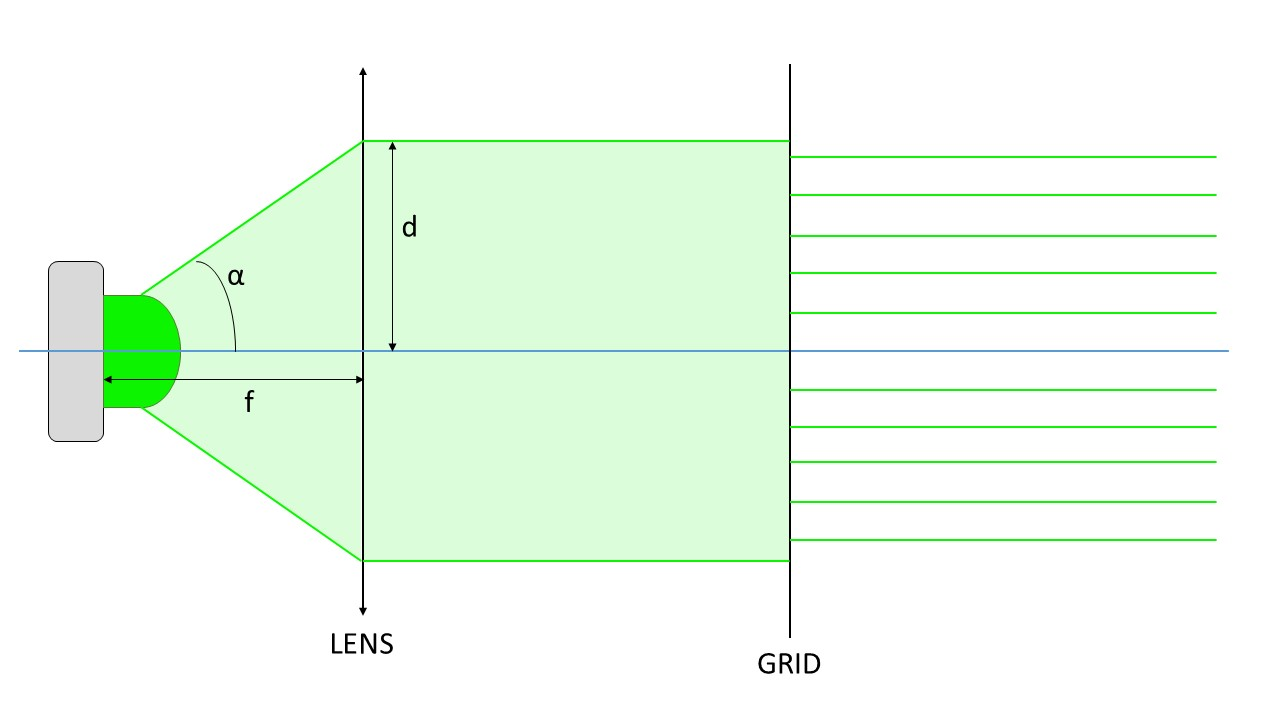
\includegraphics[scale=0.4]{fig/LEDsystem.jpg}}
  \caption{schema of the LED system}
  \label{fig:LEDsystem}
\end{figure}

As the LED has a diffusion angle of 30\textdegree (Annex \ref{LEDdatasheet}), the lens needs to be close enough to collect all the light beams of the LED to avoid losses of energy. In order to capture as much light as possible, the diameter of the lens should follow \eqref{eq:lenseLED}.

\begin{equation}
\label{eq:lenseLED}
d = f \tan \alpha
\end{equation}
with 
\begin{align*}
\alpha & = \frac{30}{2} = 15\mbox{\textdegree, the half of the diffusion angle.}\\
f & \mbox{, the focal length of the lens}
\end{align*}

Moreover, it should be pointed that there is a loss of energy because of the lens and the grid. We will assume that the energy loss coefficient of the lens $LFLLed$ (Loss Factor Lens Led) is 0.5 and the one of the grid $LFGLed$ (Loss Factor Grid Led) is 0.3.

\subsubsection{Validation of the Light Source}
\label{light Power}
~\\
In order to verify weather our light source has enough power or not to outshine the sunlight, the Signal/Noise ratio (SNR) has to be calculated (see part Signal/Noise ratio \ref{thirdcase}). Knowing that 100 is a really great SNR, as the SNR of images recorded with this system is $[32, 348]$, it can be concluded that the LED can be chosen as light source. Indeed, even if 32 is a low ratio, it is only when all the different poor conditions happen in the same time and it does not happen frequently. Moreover, 100 to 347are really high ratios that permit to have the 3D algorithm working well. Thus, the design of the light source is validated.





\subsection{Signal Noise Ratio}
First of all, the irradiance $F$ of the light from the sun falling at the top of the atmosphere of Mars can be calculated as following :
Conservation of energy :
\begin{equation}
\label{eq:conservation of energy}
4\pi R_\odot^2F_\odot=4\pi R^2F
\end{equation}
with 

$R_\odot=6,956.10^8\ m$ : solar radius

$F_\odot=6,45.10^7\ W.m^{-2}$ : energy flow of the surface of the sun

$R \in [2.06644,\ 2.49228].10^{11} \ m$ : distance Mars-Sun (Aphelion and Perihelion)

\begin{equation}
\label{eq:Irradiance Sun range}
F = F_\odot \left(\frac{R_\odot}{R}\right)^2 \in [502, 730]\ W/m^2
\end{equation}

In this report, we will consider that the rover is working on a specific date and we will chose the one when $R$ corresponds to the semi-major axis. In this case $R=2,27936.10^{11}\ km$ and
\begin{equation}
\label{eq:Irradiance Sun}
F = 589\ W/m^2
\end{equation}



Moreover, we can assume that a part of the irradiance is absorbed by the atmosphere. Knowing that the atmosphere of Earth absorbs and scatters to space around 30\% of the incident irradiance of the Sun\cite{yamamoto1962direct}, and knowing  that the atmosphere of Mars is thinner than the one of the Earth, we will postulate that 10\% of the incident irradiance is absorbed. Thus, using \ref{eq:Irradiance Sun} the actual irradiance $F_a$ of the light from the sun falling on the surface of Mars is

\begin{equation}
\label{eq:Actual Irradiance Sun}
F_a = \frac{90}{100}F = \frac{90*589}{100} = 530\ W/m^2
\end{equation}

However, this irradiance is the one of surface exposed perpendicular to the sun's beams. As Mars is a sphere, the projection need to be considered.
Knowing that the weather is better into the northern hemisphere of Mars\cite{wiki:weather} and the fact that a latitude between 30 an 70 degrees is favored for a landing\cite{latitude}, we will assume that the rover has a latitude of 50\textdegree. This latitude corresponds to an angle of 40\textdegree$\ $between the surface of Mars and the sun's beams. Moreover, suppose that the rover stop working when this angle is inferior to 10\textdegree. Thus, the irradiance $F_{50}$ at a latitude of 50\textdegree$\ $is

\begin{equation}
F_{50} = F_asin(angleBeams) \in [92, 341] \ W/m^2
\end{equation}

with $angleBeams = [10, 90-latitude] = [10, 40]$\textdegree.


Then, considering the trajectory of the Sun into the sky of Mars and knowing that the rock target is more or less vertical to the surface of Mars, the angle $\theta$ between the target's normal and the sun's beam is considered to be included in $[10, 50]$\textdegree. In addition, in the optimal case (when all the optimal conditions are provided to have the maximal radiance), the BRDF of the surface of the target is assumed to be 90\% Lambertian and 10\% Glossy while in the worst case the BRDF will be only Lambertian. In this way, the radiance of the target $R_T$ is

\begin{equation}
\label{eq:Radiance Target}
R_T = \left\{
	\begin{array}{ll}
		\frac{F_{50}\alpha}{\pi}\cos \theta & \mbox{ optimal case} \\
		F_{50}\alpha(\frac{9}{10\pi}\cos\theta + \frac{1}{10}) & \mbox{ worst case}
	\end{array}
\right.
\end{equation}

with 
\begin{align*}
	\alpha & \in [0.05, 0.45]\mbox{, the albedo of the target\ref{albedo}} \\
	\theta & \in [10, 50]\mbox{\textdegree, the angle between the target's normal and the sun's beam}
\end{align*}
Thus, 
\begin{equation}
R_T \in [92, 340] \ W/m^2
\end{equation}






\subsection{Summary and Comparison with MER Cameras}
To validate the coherence of the characteristics of the designed camera, a comparative table \ref{tabCameras} with the MER cameras Navcam (Navigation Camera) and Pancam (Panoramic Camera) \cite{merengineeringcameras} can be found below.

\begin{table}[H]
\centering
\caption{Recap chart of the Designed Camera and Comparison with Navcam and Pancam (MER Cameras)}
\label{tabCameras}
\renewcommand{\arraystretch}{1.5}
\begin{tabular}{|l|c c c|}
\hline
Features & Designed Camera & Navcam & Pancam \\
\hline
CCD &  &  &  \\
Pixel size & $12 \times 12 $ microns & $12 \times 12 $ microns & $12 \times 12 $ microns \\ 
Resolution & $1024 \times 1024 $ & $1024 \times 1024 $ & $1024 \times 1024 $ \\ 
Spectral range & [400 - 800] nm & [600 - 800] nm & [400 - 1100] nm \\ 
Readout noise, 55$\degree$ & 25 electrons & 25 electrons & 25 electrons \\
\hline
Optical properties & & &  \\
Focal length & 12.14 mm & 14.67 mm & 43 mm  \\
Entrance pupil diameter & 1.9 mm & 1.25 mm & 2.18 mm  \\
FOV & $26.6 \degree \times 26.6\degree$ & $45 \degree \times 45\degree$ & $16 \degree \times 16\degree$ \\
Depth of field & 0.67 - 2 m & 0.5 m - infinity & 1.5 m - infinity \\ 
Best focus & 1 m & 1 m & 3 m \\
\hline
\end{tabular}
\end{table}

The CCD parameters are similar except for the spectral range. As Pancam mission is to investigate Mars terrain and obtain color images of any information useful to learn more about the Red Planet, that seems logical that the spectrum is wider than the one we choose. The navigation camera provides a 360$\degree$ view of the area where is located the rover. The spectrum was reduced using filters to allow a higher spectral responsivity.
For the optical features, it can be noticed that the parameters have approximately the same size. The depth of field for our camera is restricted but it is due to our aim: stabilizing the camera in front of a rock and carrying out its depth map.
We can conclude that since the MER cameras accomplish well their task, the designed camera which is comparable to them should also be capable of acquiring good images on Mars.

\subsection{Cost and Power Consumption}
The price of a camera depends of its characteristics, especially, of the CCD sensor. The chosen one has large pixels and hence will capture more light than another CCD with half of our pixel size. That means that its performance should be better and thus, the designed camera could be quite expensive. As the exact cost of high quality camera is often not provided, and as finding a similar model to the one planned above is very difficult, it is decided to only determine a price range. Some websites such as ThorLabs have CCD cameras with a resolution of one Megapixel but with half the pixel size desired. As their cost is between 5.000 and 9.000 \euro, we estimate our camera at around 10.000 \euro. Knowing that the Nasa has planned a budget of \$1.5 billion for the new Mars Rover Mission of 2020, this price represents only $0.73\cdot 10^{-3} \ \%$ of the total mission. Taking into consideration that the fee for the artificial source (LED and lens) is negligible compared to the camera cost, it can be concluded that the amount of money needed for buying the designed camera is reasonable.

Regarding the power consumption of our system, it is assumed that the camera could be powered with 2.15 Watts since it is sufficient for supplying the MER Cameras. On the other hand, according to its datasheet (Appendix \ref{LEDdatasheet}), the LED consumption is of 220 mW. On the report of the NASA, a Martian rover needs around 100 Watts and they are provided by solar panels and rechargeable Lithium batteries. The system will then use around 2.4 \% of the rover power. It is tolerable since the camera will not take pictures all the time. It can be argued that the processor consumption should be added. However, the other actions of the robot are also controlled by the CPU, so it is not taken into account here, since it is hard to quantify the power utilized by the algorithms to compute the depth mapping.
\section{Distance Camera-Target of One Point}
Before starting to establish a whole 3D mapping, a more simple case can be studied first and it will be shown, in this section, how to determine the distance to only one point. Indeed, the distance between the camera and a point of the target can be easily determined thanks to a little bit of trigonometry.

The context of this case is simple, the camera is recording images of the target while the artificial light source is projecting a point one the last one (see figure \ref{fig:schema1D}).

\begin{figure}[h]
  %\centering
  \centerline{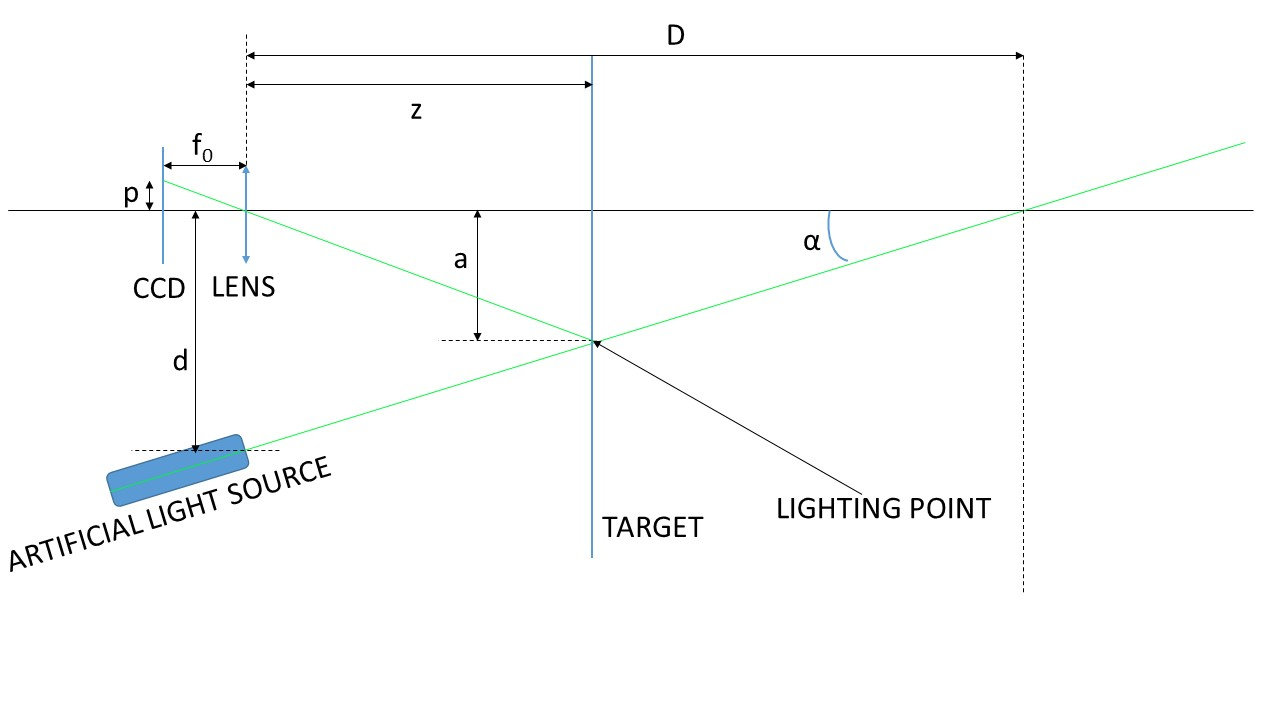
\includegraphics[scale=0.5]{fig/schema1D.jpg}}
  \caption{schema of the camera recording images of the target on which there is a lighting point from the artificial light source}
  \label{fig:schema1D}
\end{figure}

According to the figure \ref{fig:schema1D}, 
\begin{itemize}
\item \textbf{d} is the distance to determine.
\item $\bm{\alpha}$ is the angle between the focal axis of the camera and the focal axis of the light source.
\item \textbf{a} is the distance between the focal axis of the camera and the lighting point.
\item \textbf{D} is the distance between the camera and the lighting point when this one is on the focal axis of the camera.
\end{itemize}
Thus, we have

\begin{equation*}
	d=D-\frac{a}{\tan \alpha}
\label{eq:formule_1D}
\end{equation*}

However, $\bm{\alpha}$, \textbf{a} and \textbf{D} are not known yet, that is why a calibration phase is needed (see Figure \ref{fig:calibration}). The first parameter, $\bm{\alpha}$, is determined during the installation of the light source and the camera on the rover. Then, during the calibration, two steps can be identified. During the first one, a target is positioned such as the lighting point is on the center of the image recorded by the camera. Thus, \textbf{D} can be measured. During the second step, a target is positioned such as the lighting point is right on side (left or right) of the image recorded by the camera (see Figure \ref{fig:calibration}). Therefore, $a_0$ can be measured and we have

\begin{equation*}
	a = \frac{Na_0}{A_0}
\end{equation*}


with \begin{itemize} \item $N\ [pixels]$, the number of pixel between the center of the image recorded by the camera and the lighting point.
\item $A_0$ $[pixels]$, the number of pixel between the center of the image recorded by the camera and the lighting point during the calibration phase, that is to say, the half of the pixels of the width of the image.
\end{itemize}

Therefore, we have
\begin{equation}
	d=D-\frac{Na_0}{\tan \alpha}
\label{eq:formule1D}
\end{equation}

\begin{figure}[H]
  %\centering
  \centerline{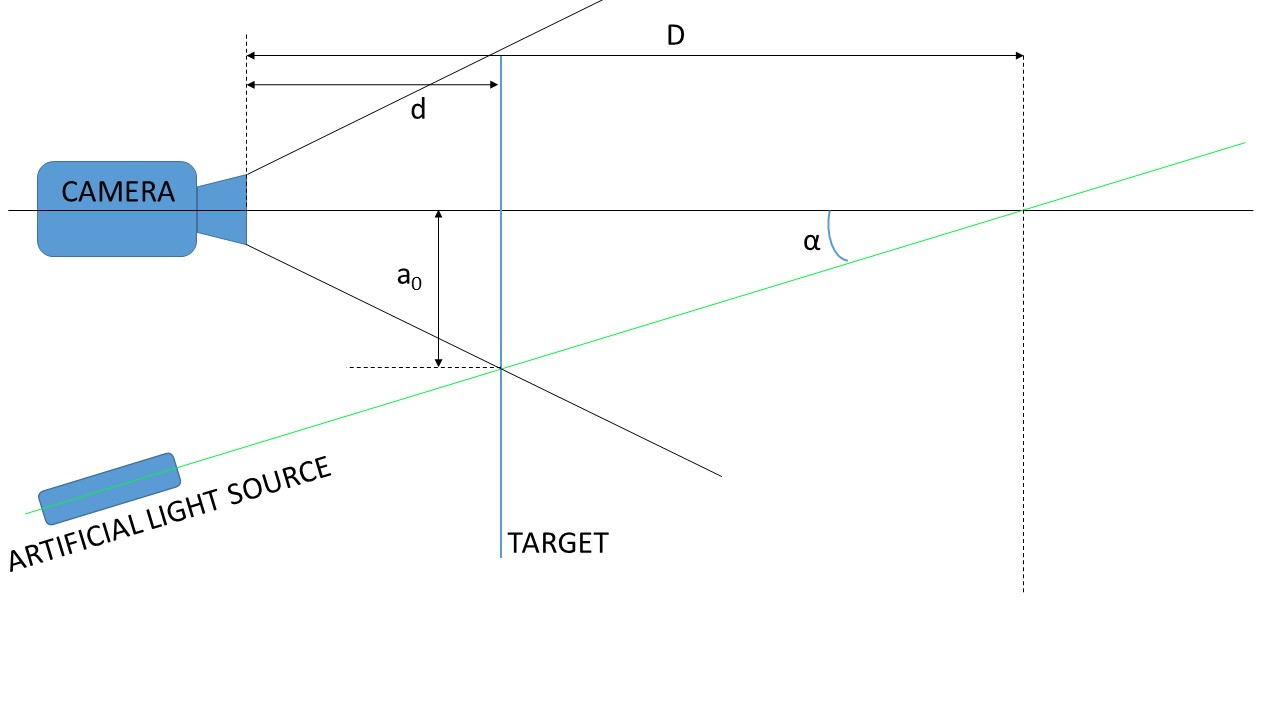
\includegraphics[scale=0.4]{fig/calibration.jpg}}
  \caption{schema of the calibration}
  \label{fig:calibration}
\end{figure}


However, a calculation of the distance camera - target using simpler calibration can be found thanks to triangulation. Indeed, using the Thales' theorem such as $\frac{z}{f_0} = \frac{a}{p}$ (see Figure \ref{fig:schema1D_2}), it can be determined that the distance \textbf{z} camera - point on the target is


\begin{equation}
z = \frac{f_0d}{p+f_0 \tan \alpha}
\label{eq:formule1D_2}
\end{equation}

Thus, only the first step of the calibration is needed because only $\bm{\alpha}$ and \textbf{d} need to be determined. $\bm{f_0}$ is a characteristic of the lens and \textbf{p} is determined thanks to the CCD characteristics ($p = p_{pixels} \frac{12,288.10^{-3}}{1024}$).

\begin{figure}[H]
  %\centering
  \centerline{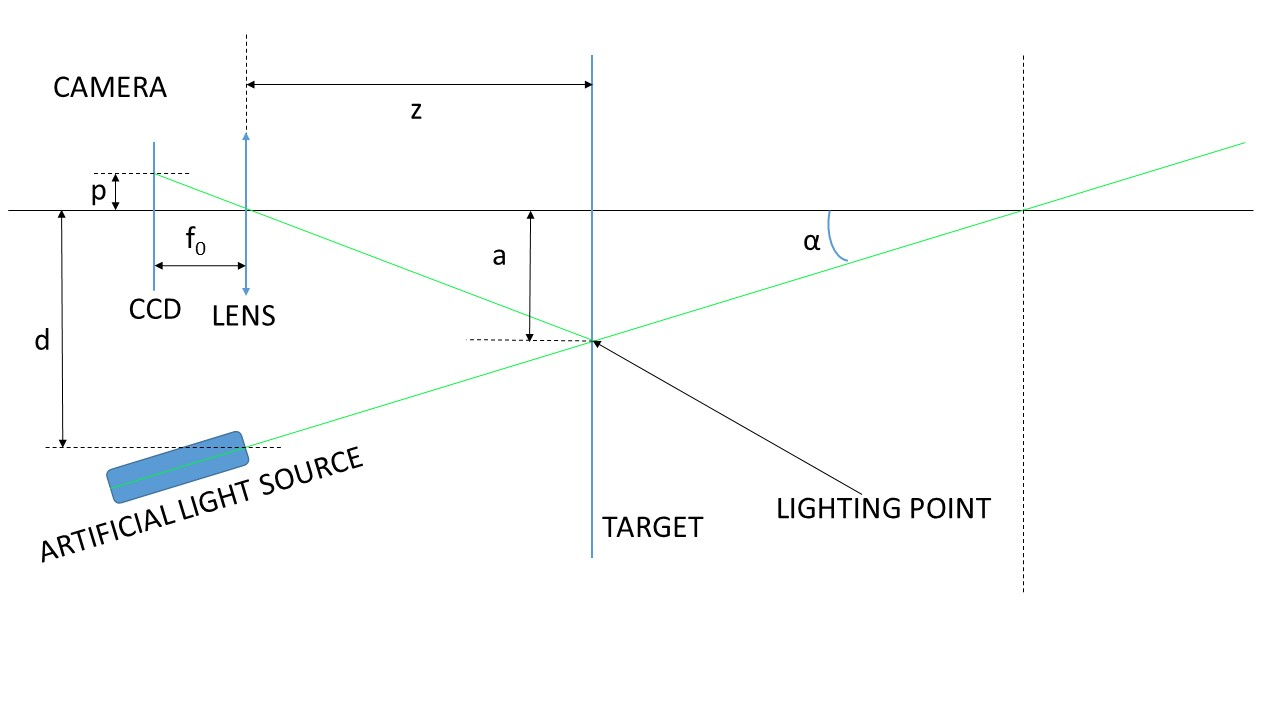
\includegraphics[scale=0.5]{fig/schema1D_2.jpg}}
  \caption{schema of the CCD sensor - lens sytem recording images of the target on which there is a lighting point from the artificial light source}
  \label{fig:schema1D_2}
\end{figure}
\section{3D Map}
In order to find the 3D map of the target, we use the triangulation method seen in the previous section on a grid of lighting points. To do so, for each lighting point, we have to use two different angles $\bm{\alpha}$ and $\bm{\beta}$. Previously, $\bm{\alpha}$ was the angle between the focal axis of the camera and the beam but now it is the angle between the focal axis of the camera and the beam projected on the plane y=0 and $\bm{\beta}$ is the angle between the focal axis of the camera and the beam projected on the plane x=0 (see figure \ref{3dmap}). In the same way, the distance \emph{d} camera-artificial light of source becomes $\bm{d_x}$ and $\bm{d_y}$.

\begin{figure}[H]
  %\centering
  \centerline{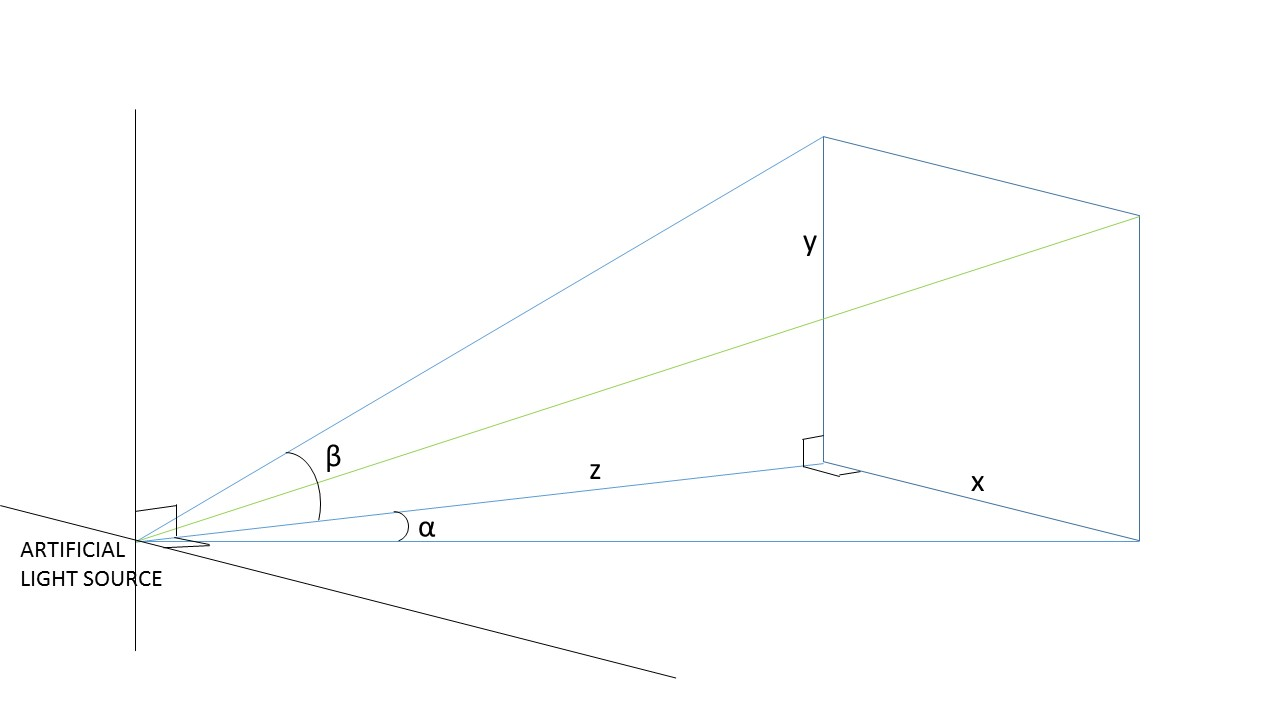
\includegraphics[scale=0.4]{fig/3dmap.jpg}}
  \caption{schema of a beam of the artificial light source}
  \label{fig:3dmap}
\end{figure}

Thus, the new distance camera-target is

\begin{equation}
z = \frac{d_x}{p_{pixels,x}\frac{P_{size}}{f_0}+ \tan \alpha}
\label{eq:formule3D}
\end{equation}

Then, to find the (x,y) coordinates of the point, we have

\begin{align}
x & = z \tan \alpha - d_x \\
y & = z \tan \beta - d_y
\end{align}

We subtract $d_x$ and $d_y$ in order to change from the artificial light source system of axis to the camera system of axis.
\section{Image Processing}
To carry out the 3D map of a Martian rock, the coordinates of the points which are projected by the LED on its surface need to be determined on the images acquired by the camera. They are obtained by detecting the points thanks to their color, by distinguishing them, and by applying the centroid algorithm to get their center. First, the color detection method will be addressed, before focusing on the differentiation and the centroiding.

\subsection{Color Detection}

To increase the robustness of the algorithm, the color of the light beams was chosen to have the maximum contrast with the color of the rock. Mars having a reddish color, a bright green light seemed adapted. Moreover, as it is explained in the scene analysis part, the CCD sensor is more sensitive to the wavelength corresponding to the green (around 520 nm). Thus, the color detection algorithm aims to find bright green spots in the camera video stream in real time. It is implemented in C with OpenCV library. 

For unit testing, the image analysis is performed by extracting frames from the video stream obtained thanks to the computer webcam. These images are processed very quickly, which allows a real time analysis. The details of the method employed are given below. For the explanation, the figures are obtained for the detection of a blue box (the H value was changed for this purpose), but the algorithm works similarly for green light beams.

To begin with, a low-pass filter is applied to the image to handle to smooth it and to reduce the noise. Once achieved, the image is converted from RGB to HSV (see Theory Section) in order to get a better control of the colors and intensities of the image pixels. The range of the HSV parameters can be determined to isolate the bright green pixels from the rest of the image. The equivalent hue is between 60\degree  and 180\degree, taking a large scope to be sure to isolate the good color component. As the luminous points will be bright, the range of the saturation and the luminosity should be chosen around the upper values. To adjust the values, several trackbars are added to the image, see figure \ref{fig:trackbars} and the modifications are made in real time. All the values under the thresholds defined are irrelevant. Thus the pixels of the binary image which corresponds to the HSV thresholding are set to 1 (white) for the zone where the light green points are recognized and to 0 (black) for the background, the rest of the image. This image is then easier to deal with because it is only composed of two values, black and white. Erosions and dilations can be applied respectively to separate connected light beams and remove noise or to fill holes in the points. The number or erosions and dilations are selected thanks to trackbars once again (figure \ref{fig:trackbars}) and they are computed with the OpenCV functions with a 3x3 rectangular structuring element. The size of the kernel of the low-pass filter is also controllable with the trackbars. 

\begin{figure}[H]
  \centering
  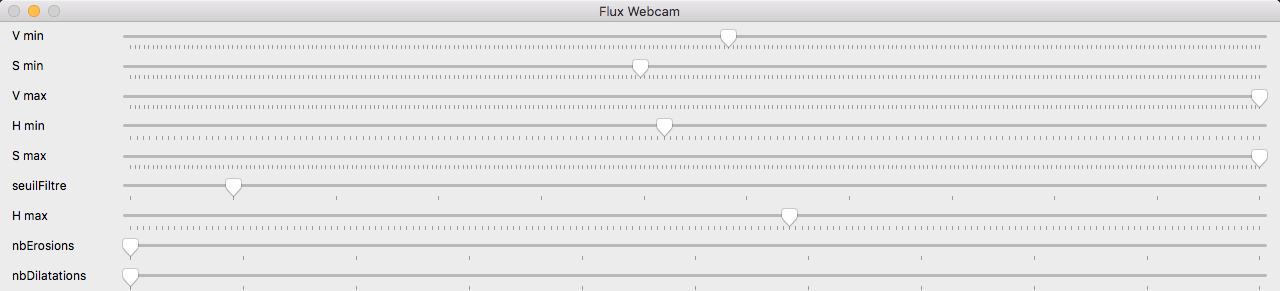
\includegraphics[scale=0.35]{fig/trackbars.png}
  \caption{Trackbars for the threshold of the filter, the HSV parameters and the number of erosion and dilation}
  \label{fig:trackbars}
\end{figure}

The calibration is carried out through the trackbars and the result is displayed on the video stream with the addition of contours to facilitate the tuning (figure \ref{fig:contours}). \textit{cvFindContours} is used to search the contour of the light spots. The detection is based on the same principle that it has been seen during the exercises in the lab. The algorithm looks for the first pixel belonging to the point and then follows the contour pixel by pixel. Once the threshold of the low-pass filter, the HSV values and the number of erosion and dilation are established, the calibration is completed. For the unit testing with the blue box, we only focus on the color detection and the centroiding. Thus, no erosion nor dilation are added and the filter kernel is set to one pixel, which does nothing. 

\begin{figure}[H]
  \centering
  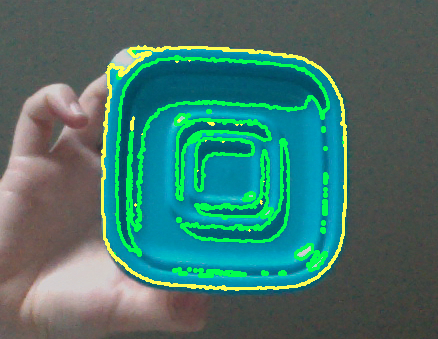
\includegraphics[scale=0.6]{fig/contours.png}
  \caption{Contours of the detected object}
  \label{fig:contours}
\end{figure}

In order to compute the centroid of the beams spots, it is needed to retrieve their intensity. To this end, the color detection should return an image with the light points in HSV color on a black background. To do so, the binary image is multiplied by the HSV image. The multiplication is explained by the pseudo code below.\\

\begin{algorithmic}
\Function{multiplication}{binary image, color image}
	\For{each pixel in the binary image}
		\If {the pixel value is white}
    			\State $pixelHSVColor \gets$ the color of the pixel in the HSV image
    			\State the color of the pixel in the final image $\gets pixelHSVColor$
		\Else
        			\State the color of the pixel in the final image $\gets$ black color
		\EndIf
	\EndFor
\EndFunction
\end{algorithmic}

The final image obtained is shown figure \ref{fig:finalImage}. Each white pixel corresponding to 1 in the binary image is replaced in the final image by the HSV value of the original image and the background is set to black like in the binary image.

\begin{figure}[h]
  \centering
  
\includegraphics[scale=0.6]{fig/finalImage.png}
  \caption{Object detected in HSV color system on a black background}
  \label{fig:finalImage}
\end{figure}

\subsection{Beams Distinction}
In the previous part, a unit test was performed with a blue box to check the efficiency of the color detection algorithm. However, the aim is to project a grid of 10 x 10 green points on a rock. Once they are extracted from the rest of the image with the same technique described above, they need to be separated. Indeed, for now, we only have the coordinates of the pixels assumed to belong to the beam spots. To look for their center of mass, the pixels which constitute each point have to be gathered. 

It should be noticed that, as no pattern other than an unicolor grid is used to carry out the depth mapping, the green points cannot be distinguished from each others. Thus, this implementation does not take into account the position of each beam spot, which could be problematic if the deformation is too important. Indeed, if a point is slightly linked to another or if it has moved and is a bit above or under the others, it is still possible to retrieve its original position. It is only if the change is too important (permutation of dots for example), that it will be very complicated to get the correct location of each beam spot. To solve this problem, a solution is described in the Pattern Disorders paragraph \ref{PatternDisorders} in the Theory Section, which would assure that no spot has been switched. Nevertheless, this method requires a pattern projection and is dismissed in a first approach. 

To differentiate each point, a recursive method was implemented using C++ which consists to isolate a point using neighbouring pixels. The pseudo code explaining the technique can be found below:\\

\begin{algorithmic}
\Function{findPointRec}{table, pixel, information to scan the image}\\
\Comment{table contains the coordinates of the pixel belonging to the current point}
		\If {the pixel value is is not black}
    			\State add to $table$ the $pixel$ coordinates and its value
    			\State the $pixel$ value in the image $\gets$ 0
			\State findPointRec(table, left neighbouring pixel, image information)
			\State findPointRec(table, right neighbouring pixel, image information)
			\State findPointRec(table, above neighbouring pixel, image information)
			\State findPointRec(table, below neighbouring pixel, image information))
		\EndIf
\EndFunction
\end{algorithmic}

The image is scanned and it is assumed that a new point begins each time that a green pixel is detected. A table to collect the coordinates of pixels belonging to the new beam spot is created and given in parameter to the recursive method. The first pixel position is added to the table, its value is set to 0 in the image and the recursive method is repeated while neighbouring pixels are found. At the end, a 2D table is obtained where the rows correspond to the spots and the columns to each pixel belonging to the point. The centroiding algorithm can then be processed to determine the center of mass of each spot and compute their distance to the camera. We can note that, for now, the points are separated but if they were not perfectly aligned on the projection, the rows of the 2D table are not in the same order than the original projected points.
\subsection{Centroiding}

The 3D map can be performed with the coordinates of the light beams seen by the camera. They are determined by estimating the center of the spot, and to do so, the center of mass, also called the centroid needs to be calculated in the final image acquired by the color detection. In order to get it, a barycenter of the pixels belonging to the ray is carried out weighted by the intensity of the pixel (S value in HSV model).

\begin{align}
x_c &= \frac{\sum_x x \cdot I(x,y)}{\sum_x \sum_y I(x,y)} \label{xcentroid} \\
y_c &= \frac{\sum_y y \cdot I(x,y)}{\sum_x \sum_y I(x,y)} \label{ycentroid}
\end{align}
Where $x_c$ and $y_c$ are the coordinates of the center of mass of the beam, $x$ and $y$ the coordinates of each pixel belonging to the beam and $I$ their corresponding intensity.

The intensity of each pixel is obtained by splitting the canals of the image into three to retrieve an image with only the Saturation values. Then the formulas \eqref{xcentroid} and \eqref{ycentroid} are computed. A white cross is displayed on the centroid as it can be seen on the figure \ref{fig:finalImage}. The computation was performed for the same box as in the color detection but the algorithm can be adapted for several beams.

%results section
\chapter{Experimental Results}
To validate the system and algorithms previously defined, several integration tests are carried out. The camera used and the additional source of light are not the same as the one described above, and they are performed on Earth, thus the verification of the system will not be complete. Nevertheless, it will be enough to, at least, confirm that the approach is achievable and needs to be further investigated. 

\section{Equipment Employed for the Experiments}
To carry out the experiments, we should build the system designed in the previous part. However, to saving time and money, it is decided to use an alternative equipment, easier to obtain, with a behavior similar to the chosen one. The components of the new system are described below.

\subsection{Lab Webcam Philips SPZ2000}
First, to carry out all the experiments, a camera to acquire the images of the scene is needed. As the camera designed in the Scene Analysis have to be built with expensive constituents, and we didn't have a lot of time, it was decided to use the webcam in the lab as a substitute. They are not accurate and their image is blurred when the object to focus is too far from it but if the algorithms compute the right distances with such a camera, a more advanced one will be capable to obtain the same or even more precise results. However, some information such as the focal length and the pixel size of the CCD are unknown. A preliminary calibration to determine the focal length and the lens distortion will be achieved before performing the experiment.

\subsection{Laser Pointer}
To simulate the additional source of light, a laser pointer is used. Only one beam is needed to perform the experiment, thus no other system will be added to split the ray. The wavelength of the laser is 532 nm, like the color chosen in the design part. Its maximum output power is 5 mW which corresponds to the order of magnitude selected before. It may not be enough to outshine the sun, but it is adequate for checking the algorithms indoor. It is powered with batteries which will not be adapted on Mars as the rover should be autonomous. 

\subsection{Computer}
On the rover, it is a micro-controller which will provide the computational power to carry out the image analysis and the calculation of the distance of the beam spots detected. As we are only testing the algorithms, and not implementing the whole system designed, a computer connected to the webcam to retrieve the images acquired is used. 

\section{Parameters of the Webcam}
As the datasheet of the webcam employed to carry out the experiments is not exhaustive, we need to establish its focal length and the impact of the lens distortion.

\subsection{Determination of the Focal Length}
Two techniques are used to find the focal length: the triangulation method and the Matlab Camera Calibration Toolbox \cite{matlabtoolbox}.

\subsubsection{Triangulation Method}
The first approach consists in placing an object whose size is known at a certain distance of the webcam and in taking a picture of it. The figure \ref{fig:schema1D} can be taken as a reference, where z is the distance camera-object, a the size of the object, p the size of the object in the image plane and $f_o$ the focal length that we want to determine. With the Thales' Theorem, it is deduced:
\begin{equation}
\frac{f_0}{z} = \frac{p}{a}
\label{eq:focal}
\end{equation}
As we measure the size of the object in the image plane in pixels, it is needed to convert it in meters. Thus, the size of each pixel of the CCD has to be known, which is not the case since the datasheet does not provide this information. However, by looking at the formula \eqref{eq:formule1D_2}, it can be noticed that we need the ratio $\frac{Pixel Size}{f_0}$ and not $f_0$ alone. This means that by deriving \eqref{eq:focal} using $p = P_{pixel} \times Pixel \ Size$ on the \textbf{x} direction, we obtain our desired ratio:
\begin{equation*}
\frac{Pixel \ Size}{f_0} = \frac{a}{Z \times P_{pixel}}
\end{equation*}

The ratio is calculated for an object of 1 m, at a distance of 5.21 m, which corresponds to 147 pixels in the image plane. It is equal to $0.0013 \ pixel^{-1}$ . This ratio is used to compute the distance object-target in the experiments but as it depends a lot of parameters measured by hand, another solution, more accurate as it is based on the cross correlation of several images is considered. 

\subsubsection{Camera Calibration}
Camera features, which include the focal length, can be obtained thanks to the Matlab Camera Calibration Toolbox \cite{matlabtoolbox}. Several pictures of a checkerboard are taken, changing the orientation of the checkerboard and its position in the image. The Matlab Single Camera Application App analyses these images and detects the intersections between four squares of the checkerboard as it can be seen in green on the figure \ref{fig:checkerboard} (Appendix \ref{Toolbox}). The origin is in yellow. Once this step achieved and the real size of one square known (39 mm here), the camera intrinsics, extrinsics and lens distortion parameters are estimated by a technique called geometric camera calibration. It uses the intersections coordinates of the checkerboard in different configurations and the factor scale to model the camera by a camera matrix which permits to transform the world coordinates into pixel coordinates on the image plan.

\paragraph*{Extrinsics Parameters}
~\\
The extrinsics parameters composed of a rotation matrix and a translation convert the world coordinated into the camera coordinates. As we are already doing this computation with our own method, these parameters are not relevant for us. Nevertheless, it can be noticed (see figure \ref{fig:extrinsics} in Appendix \ref{Toolbox}) that the Matlab functions locate accurately the position of the checkerboard. The Z coordinate is found to be around 1 m 40 and that is at that distance that the experiment was performed. Their angle seen by the camera is also precise. The correlation between several images is proved to be efficient to find the distance of a geometric image but it is not feasible on Mars soil.

\paragraph*{Intrinsics Parameters}
~\\
The intrinsics parameters are composed of the focal length and of the coordinates of the optical center in the image plan (see Table \ref{intrisicsPara}). The focal length is given in pixels in the X and Y directions. 

\begin{table}[H]
\centering
\caption{Intrinsics Parameters with Estimation Errors}
\label{intrisicsPara}
\renewcommand{\arraystretch}{1.5}
\begin{tabular}{|c|c|c|}
\hline
Intrinsic Parameters & Focal Length (in pixels) & Optical Center (in pixels)\\ \hline
Direction x & 826 $\pm$ 33 & 378 $\pm$ 29 \\ \hline
Direction y &  805 $\pm$ 31 & 175 $\pm$ 34 \\ 
\hline
\end{tabular}
\end{table}

As $f_x = \frac{f_0}{Pixel \ Size_{\text{x}}}$, we can compare the ratio previously calculated thanks to measurements to the $f_x$ found by calibrating the camera with the Matlab Toolbox. Taking into account the errors:
\begin{equation*}
Ratio = \frac{1}{f_x} \in \ [0.00116 \quad 0.00126] \ pixel^{-1}
\end{equation*}

Taking the mean of this fraction, the error between the two ratios is of 7 \%. As even the ratio with the Matlab Toolbox is not accurate since the lower bound is increased by 8.7 \% to get the upper bound, it is decided to use this calibration ratio for 1 beam spot integration testing only. Regarding the experiment with a row of points, as it was carried out for the same distance as the focal length computed by the triangulation method, the first ratio is kept. 

\subsection{Discussion About the Lens Distortion}
The smaller the lens is, the more is the chance that lens distortion occurs. The Toolbox allows us to consider the radial and tangential distortions. According the the documentation \cite{matlabtoolbox}, the latter "occurs when the lens and the image plane are not parallel" and the first one "when light rays bend more near the edges of a lens than they do at its optical center". To account for the lens distortion in our model, which could permit to obtain more accurate results as the webcam could not be perfect, the two distortions are applied to the distance in pixel between the center of the image and the optical center (computed by Matlab, see Table \ref{intrisicsPara}) and between the the centroid studied and the optical center. The difference between the two distances distorted gives us the distorted distance between the center of the image and the centroid, used to calculate the depth map. The formula to find the distortion  in the \textbf{x} direction can be found below:
\begin{equation}
\text{x}_{distorted} = \text{x}(1 + k_1 \cdot r^2 + k_2 \cdot r^4) + 2p_1 \cdot x \cdot y + p_2(r^2 + 2\text{x}^2)
\end{equation}
Where $\text{x}$ and y are the undistorted distance to the optical center, normalized by the focal length in pixel, $r^2 = \text{x}^2 + y^2$, $k_1$ and $k_2$ the radial distortion coefficients and $p_1$ and $p_2$, the tangential ones given by the Calibration App.

\section{Determination of the Depth of One Laser Beam}
In this first integration test, we would like to establish the distance from the camera to one specific point of a surface, before checking the algorithms for several points. The general procedure is detailed below. 

\subsection{General Procedure}
As the angle between the focal axis of the camera and the focal axis of the light source is easier to obtain when the laser and the camera are aligned, they need to be located on the same axis for the experiment (see figure \ref{fig:experiment1point}). Once they are placed, the distance \textbf{d} between them is measured. Then a surface is required to project the laser beam. As it is more convenient to have a mobile surface to be able to move easily the target, we choose to use a blackboard for the test (figure \ref{fig:blackboard}). The green is dark enough to contrast with the light green spot and the albedo of this surface is not very important which illustrates one of the worst case of the reflective power of a martian rock. The distance from the blackboard to the camera is measured to calibrate the system.

\begin{figure}[!h] 
\centering
\subfigure[System Camera-Laser]{
  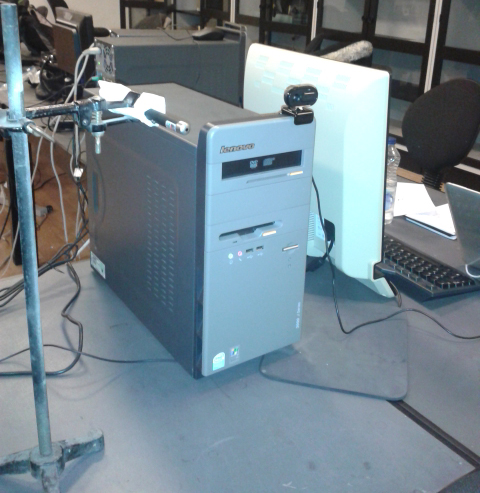
\includegraphics[scale=0.35]{fig/CamLaser.jpg}
  \label{fig:experiment1point}
}
\quad 
\subfigure[Blackboard]{
  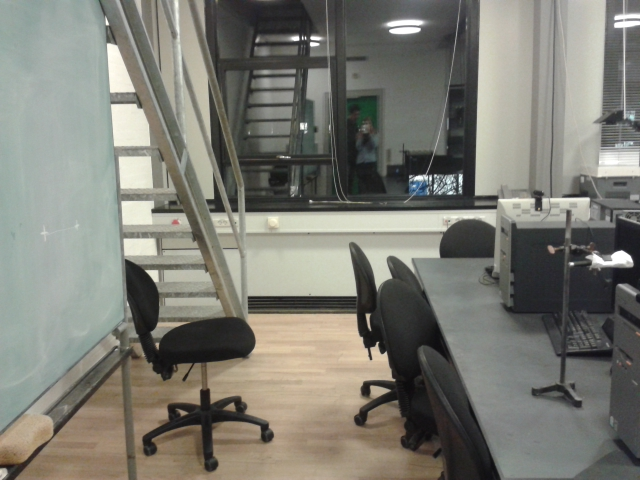
\includegraphics[scale=0.35]{fig/BlackBoard.jpg}
  \label{fig:blackboard}
}
\caption{System Camera-Laser-Blackboard} 
\end{figure}

\subsubsection{Calibration}
Two calibrations need to be accomplished before carrying out the 3D map of the point: setting the laser position and tuning the parameters thanks to the trackbars to detect the point.
\paragraph*{Material}
~\\
The webcam is connected to the computer and the calibration program is run. It only consists in acquiring frames from the webcam and displaying them on the screen of the computer. A cross is added in the center of each image to facilitate the calibration. The purpose of this step is to obtain the spot projected by the laser at the center of the image. Indeed, once this achieved, we get easily the angle $\alpha$ between the focal axis of the camera and the one of the light source, needed to compute the depth map. It can be deduced from the figure \ref{fig:schema1D} that $tan(\alpha) = \frac{d}{z}$, where d is the distance camera-laser and z the distance camera-blackboard.

\paragraph*{Color Detection}
~\\
Once the laser position is set, the color detection program is started. The parameters need to be tuned to detect the bright green color of the beam spot. As we are dealing with only one point, it is not imperative to add erosion or dilation to make an opening. The noise can be discarded with only the expected pixel size of the spot in the image plane. Thus, only the HSV values are changed to match the green of the point.

\subsubsection{Distance Computation}
The calibration accomplished, the distance can be calculated either in real time since frames for the webcam are acquired quickly and the processing is short, either later on, using pictures saved after the calibration steps at different positions of the blackboard.

\subsection{Experiment and Results}
The general procedure described is implemented with the distance camera-laser equals to 30 cm, the distance camera-blackboard equals to 137 cm, hence an angle $\alpha$ of 12.75~$\degree$. The experiment was carried out in real time and repeated a second time, handling only pictures and taking into account the lens distortion. This is the latter result which are given below in the Table \ref{results1Point}. They correspond to the image processing displayed on figures \ref{fig:exp1Point137} and \ref{fig:exp1Point98dot5}.

\begin{figure}[!h] 
\centering
\subfigure[Original Image (137 cm)]{
  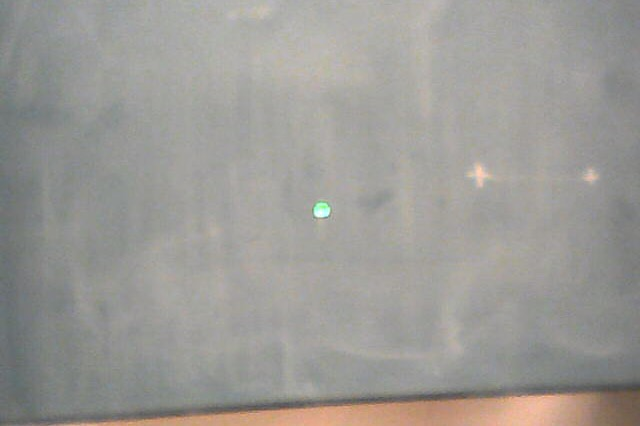
\includegraphics[scale=0.3]{fig/137cm.jpg}
  \label{fig:exp1Point137}
}
\quad 
\subfigure[HSV Image of the Point Detected (137 cm)]{
  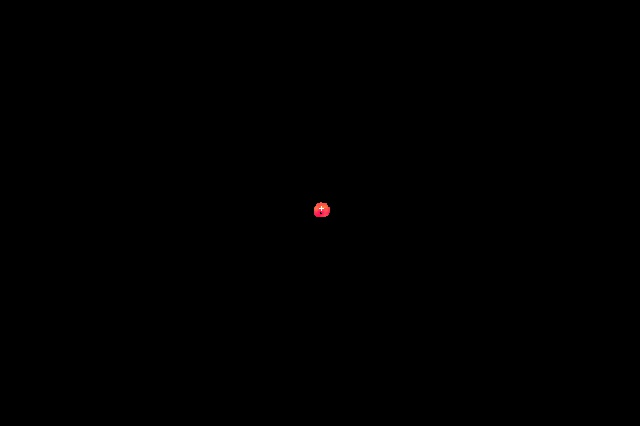
\includegraphics[scale=0.3]{fig/137PointHSV.jpg}
  \label{fig:exp1Point137HSV}
}
\subfigure[Original Image (98.5 cm)]{
  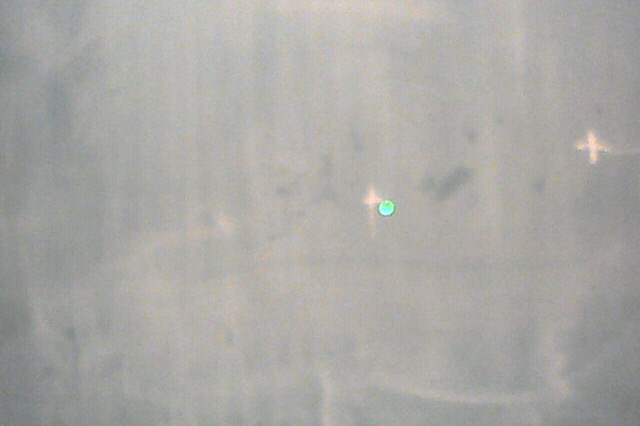
\includegraphics[scale=0.3]{fig/98dot5cm.jpg}
  \label{fig:exp1Point98dot5}
}
\quad 
\subfigure[HSV Image of the Point Detected (98.5 cm)]{
  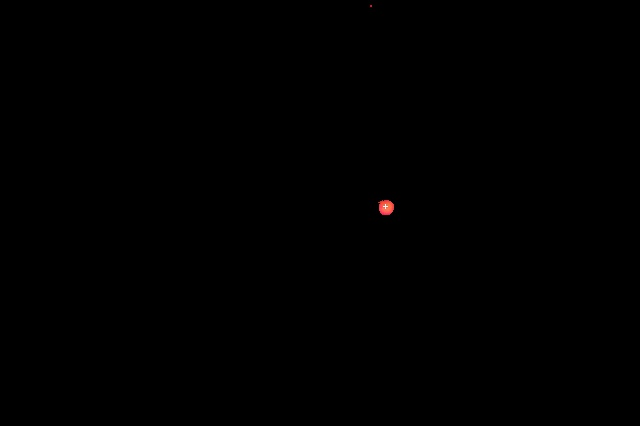
\includegraphics[scale=0.3]{fig/98dot5PointHSV.jpg}
  \label{fig:exp1Point98dot5HSV}
}
\caption{Experiment Images Acquired by the Camera and Processed for 137 cm and 98.5 cm} 
\end{figure}

\begin{table}[h]
\centering
\caption{Results of the depth mapping for 1 point with and without lens distortion}
\label{results1Point}
\renewcommand{\arraystretch}{1.5}
\begin{tabular}{|c|c|c|}
\hline
\multicolumn{3}{|c|}{Distance (cm)} \\ \hline
Camera-Blackboard & Computed without distortion & Computed with distortion \\ \hline
137 & 136.2463 & 136.2557 \\ \hline
124 & 125.2243 & 125.2153 \\ \hline
111.5 & 113.2045 & 113.1927 \\ \hline
98.5 & 100.7686 & 106.4445 \\ \hline
\end{tabular}
\end{table}

Finally, the errors with and without lens distortion are detailed in the chart \ref{chart1Point}. It can be noticed that the more the blackboard is brought closer to the camera and is moved away from its calibration position, the more the error increases. Indeed, when the blackboard is closer to the camera, the displacement of the point from the center of the image is larger (see figures \ref{fig:exp1Point137HSV} and \ref{fig:exp1Point98dot5HSV}) and the error gets bigger with the distance centroid-center of the image. Without the distortion, the inaccuracy is between 7.5 mm for 137 cm and 22.7 mm for 98.5 cm. For the latter, it is quite a large error since the rock could be nearly flat and in order to stabilize the arm, a precise 3D map needs to be carried out. If the rock relief is in the range of the millimeter, it is likely that all the results of the distances will not do any difference between several points and the stabilization could not be achieved since no specific spot could be tracked in two images acquired at different times. The errors could be caused firstly by the fact that the experimental conditions were not ideal. The distances were measured thanks to a measuring tape but the precision was only around the millimiters, and as it was not perfectly straight between the camera and the blackboard, measurement errors could occur. Moreover, the blackboard was moved several times and could have not been perfectly perpendicular to the camera optical axis. Then, the camera images were blurred and it was not designed for this kind of processing, which biased the centroiding. Also, when the point is detected, it could have less or more pixels than the original point, used for the calibration. That means that the center of mass could be displaced and create important errors. An analysis of this error will be carried out further in the report.

\begin{figure}[!h] 
\centering
  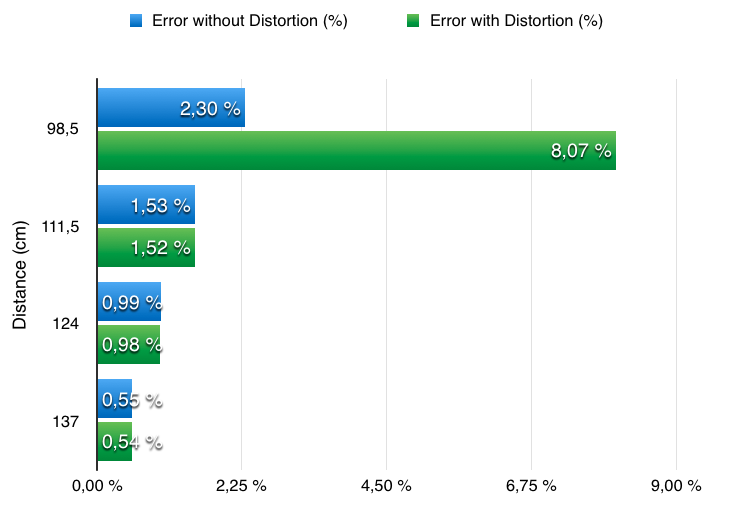
\includegraphics[scale=0.5]{fig/chart1Point.png}
\caption{Distance Errors with and without Lens Distortion} 
\label{chart1Point}
\end{figure}

Finally, the lens distortion have to be taken into account for explaining the results. Indeed, it can be observed that the error between the real distance and the computed one comes from the fact that the lens have distortions and that the distance measured between the centroid and the center of the image is inexact. To deal with this issue, the radial and tangential distortions parameters calculated by the Matlab Calibration Toolbox were added to the algorithm in order to compute the distance considering the case with the lens distortion. The results are also detailed in the Table \ref{results1Point} and the chart \ref{chart1Point}. As expected, when the distance is computed with the distance centroid-center of the image distorted, the measurement error is slightly smaller than in the case without distortion and it can be deduced that the lens distortion does not affect a lot the depth mapping. However, for the last distance, the error with distortion is not at all expected and shows either the limit of the lens distortion or that the distortion was wrongly implemented. Indeed, Matlab has estimated it for 137 cm. At this point, there were already estimation errors. As we get closer, the distorted distance increases and the errors are added. We should try to calibrate the camera at this distance or even closer and check the distortion parameters. Nevertheless, even if the error is accumulated, we should not obtain such a difference for the last distance tested. The implementation should be revised. An other solution will be to carry out this integration test with the designed camera, which should have a negligible lens distortion and be more accurate. The results should improve and the error may be tolerable.

Even if the results are not accurate and insufficient, it is a good beginning of distance approximations and with a better material and experimental conditions, they could be improved. It should also be noticed that the time of computation is low and sufficient for real time applications. Indeed, without taking into account the lens distortion, the distance is calculated in around 35 ms and when the distorted distance is also computed, the algorithms are 1 ms slower. It is now desired to find the depth of multiple points at the same time.
\section{Distances with Several Points}
After the experiment with only one lighting dot, the next step is using several lighting points. Thus, the goal of this experiment is using several points in order to detect several distances in front of the camera.

\subsection{Choices of Implementation}
First of all, a grid of dots is supposed to be projected on the target. However, instead of a grid, a line of 10 dots is used during this experiment. Indeed, as the triangulation theory between a grid of and a line of dots is the same and the indexing of the dots of a grid is much more difficult than the one of the dots of a line, it has been chosen to use a line in order to focus on the improvement of the robustness ans accuracy of the algorithm. Once these two goals completed, only the implementation of a function permitting the indexation of the dots of the grid would be needed to switch to a grid.

Then, as the purpose of this project is the vision analysis, the focus is on the structured light algorithm and the artificial light source has not been built. Thus, in order to be able to project a line of several dots on a target, it has been chosen to use a overhead projector. Indeed, even if a laser was available (see the first experiment), after trying to diffract its beam (using a CD for instance), it appeared that the brightness of each dot was very imbalanced (central dot very luminous compared to the others) and would lead to a modification of the parameters of the dot detection. Moreover, as the artificial light source is supposed to project a grid of identical dots, the overhead projector has been chosen to respect this equality of brightness.


\subsection{Progress of the Experiment}
A picture of a line of 10 green dots (a green close to the one of the laser) with a reddish background (in order to represent the color of the rocks of Mars) is projected on a board using the overhead projector. Then an object is placed between the board and the camera and the several distance $z_i$ are computed (see Figure \ref{fig:expGridSchema}).


\begin{figure}[H]
  %\centering
  \centerline{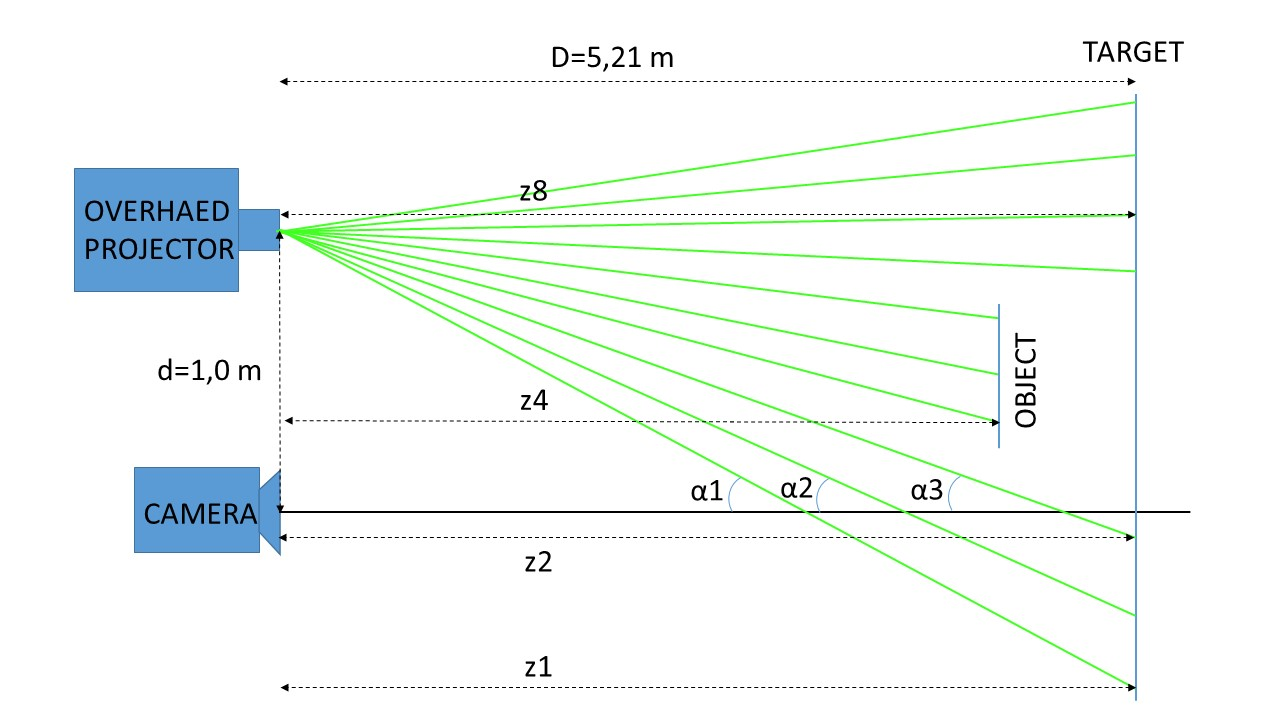
\includegraphics[scale=0.4]{fig/expGridSchema.jpg}}
  \caption{schema of the experiment}
  \label{fig:expGridSchema}
\end{figure}


Once the script is run, the different steps are the following :
\paragraph*{Step 1 : Calibration}
~~\\
In order to find the different angles $\alpha_i$ between the focal axis of the camera and the beams of the projector, a calibration function is called before the real time loop. This function detects the lighting dots, their centroid and use the following formula to save the different $\tan \alpha_i$ into an array.

\begin{equation*}
\tan \alpha_i = \frac{d}{D}-P_{pixels,i}\frac{P_{size}}{f_0}
\end{equation*}


\paragraph*{Step 2 : Positioning of the Object}
~~\\
During this step, while the script is still running, the object is placed between the camera and the board (see Figure \ref{fig:positioningObject}). On the one hand, as the projector is higher than the camera, it makes the $9^{th}$ dot slide vertically. However, it does not affect the result as only the horizontal slide is taken into account and the \emph{sort} function permits to keep the dots in the right order even if they slide vertically. On the other hand, a horizontal slide occurs as expected.

The experiment has been carried out with several distances and placing objects in front of several dots. Moreover, some noise has been added. As we can see figure \ref{fig:positioning70Object}, the background is nuanced, smaller dots with the same green are added and dots of the same size but with others greens are added too. We can see figure \ref{fig:expGrid70HSV} that the algorithm manages to filter the different noises and still detects the 10 dots.



\begin{figure}[!h] 
\centering
\subfigure[Positioning of the object in front of the $9^{th}$ dot]{
  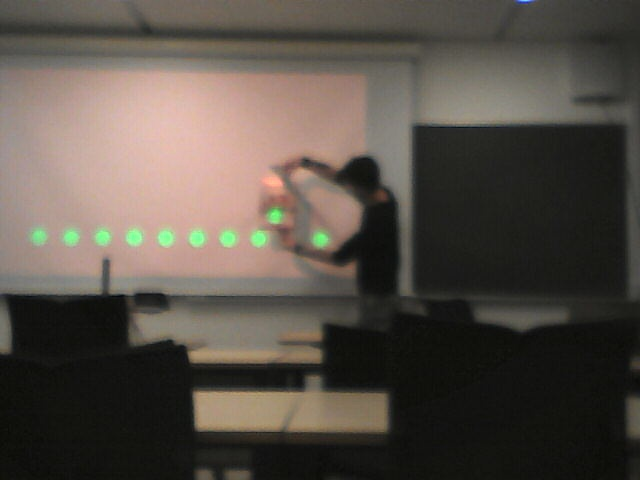
\includegraphics[scale=0.30]{fig/positioning50Object.jpg}
  \label{fig:positioningObject}
}
\quad 
\subfigure[Detection of the centroids]{
  
\includegraphics[scale=0.30]{fig/expGrid50HSV.jpg}
  \label{fig:expGridHSV}
}
\caption{Distance object-board = 50 cm}
\end{figure}

\begin{figure}[!h] 
\centering
\subfigure[Positioning of the object in front of the $6^{th}$ and $7^{th}$ dots]{
  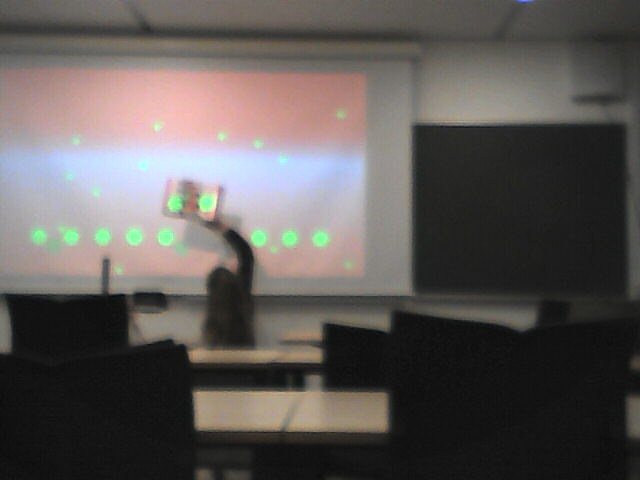
\includegraphics[scale=0.30]{fig/grid70.jpg}
  \label{fig:positioning70Object}
}
\quad 
\subfigure[Detection of the centroids]{
  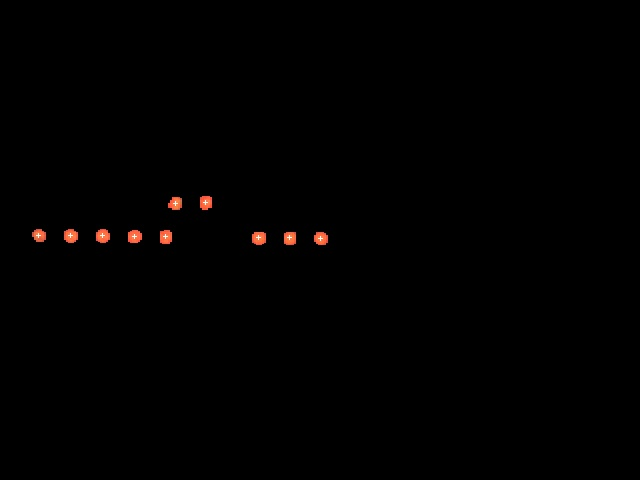
\includegraphics[scale=0.30]{fig/grid70HSV.jpg}
  \label{fig:expGrid70HSV}
}
\caption{Distance object-board = 90 cm}
\end{figure}


This experiment was carried out in real time, that is to say the several distances were displayed continuously. However, some pictures were saved in order to permit people to run the algorithm used during the experiment. Indeed, you can find into the folder '???????' the C++ script used and pictures of objects at several distances taken by the camera. Note that the script needs to be modified to use pictures instead of a video flux. Moreover, the Power Points used to project the dots and backgrounds are also present in order to permit the performing of the experiment in real time but in this case, the distances camera-projector \emph{d} and camera-target \emph{D} need to be adapted and the calibration done.


\subsection{Results}
The results of the experiment for the different distances object-board are presented Tables \ref{res50cm}, \ref{res50cm2}, \ref{res90cm} and \ref{res70cm}.

\begin{table}[H]
\centering
\caption{Object in front of dot 9 with distance object-board = 0.50 m (without noise)}
\label{res50cm}
\renewcommand{\arraystretch}{1.5}
\begin{tabular}{|c|c|c|c|c|c|}
\hline
i & $z_i$ [m] & error\footnotemark[1] [\%] & distance board-Object [m] & error\footnotemark[1] [\%] \\
\hline
1 & 5.16205 & 0.92 & 0.048 & \\
\hline
2 & 5.18899 & 0.40 & 0.021 & \\
\hline
3 & 5.20282 & 0.14 & 0.007 & \\
\hline
4 & 5.20879 & 0.02 & 0.001 & \\
\hline
5 & 5.20999 & 0.00 & 0.000 & \\
\hline
6 & 5.17524 & 0.67 & 0.035 & \\
\hline 
7 & 5.21324 & 0.06 & -0.003 & \\
\hline
8 & 5.22243 & 0.24 & -0.012 & \\
\hline
9 & 4.75529 & 0.01 & 0.455 & 9.06 \\
\hline
10 & 5.27336 & 1.22 & -0.063 & \\
\hline
\end{tabular}
\end{table}
\footnotetext[1]{$error = \frac{distance_{theory}-distance_{experiment}}{distance_{theory}}100$}

\begin{table}[H]
\centering
\caption{Object in front of dots 1 and 2 with distance object-board = 0.50 m (without noise)}
\label{res50cm2}
\renewcommand{\arraystretch}{1.5}
\begin{tabular}{|c|c|c|c|c|c|}
\hline
i & $z_i$ [m] & error [\%] & distance board-Object [m] & error [\%] \\
\hline
1 & 4.69081 & 0.41 & 0.519 & 3.84 \\
\hline
2 & 4.74072 & 0.65 & 0.469 & 6.14 \\
\hline
3 & 5.20312 & 0.13 & 0.007 & \\
\hline
4 & 5.17385 & 0.69 & 0.036 & \\
\hline
5 & 5.20999 & 0.00 & 0.000 & \\
\hline
6 & 5.2103 & 0.01 & -0.000 & \\
\hline 
7 & 5.21342 & 0.07 & -0.003 & \\
\hline
8 & 5.22243 & 0.24 & -0.012 & \\
\hline
9 & 5.24131 & 0.60 & -0.031 & \\
\hline
10 & 5.30847 & 1.89 & -0.098 & \\
\hline
\end{tabular}
\end{table}



\begin{table}[H]
\centering
\caption{Object in front of dots 1 and 2 with distance object-board = 0.90 m (without noise)}
\label{res90cm}
\renewcommand{\arraystretch}{1.5}
\begin{tabular}{|c|c|c|c|c|c|}
\hline
i & $z_i$ [m] & error [\%] & distance board-Object [m] & error [\%] \\
\hline
1 & 4.34553 & 0.82 & 0.864 & 3.95 \\
\hline
2 & 4.36417  & 1.26 & 0.846 & 6.02 \\
\hline
3 & 5.23825 & 0.54 & -0.028 & \\
\hline
4 & 5.2443 & 0.66 & -0.034 & \\
\hline
5 & 5.20999 &	0.00 & 0.000 & \\
\hline
6 & 5.17524 &	0,67 & 0,035 & \\
\hline
7 & 5.21324	& 0,06 & -0,003 & \\
\hline
8 & 5.22243	& 0,24 & -0,012 & \\
\hline
9 & 5.27727	& 1,29 & -0,067 & \\
\hline
10 & 5.23746 & 0,53 &	-0,027 & \\
\hline
\end{tabular}
\end{table}


\begin{table}[H]
\centering
\caption{Object in front of dots 6 and 7 with distance object-board = 0.70 m and noise}
\label{res70cm}
\renewcommand{\arraystretch}{1.5}
\begin{tabular}{|c|c|c|c|c|c|}
\hline
i & $z_i$ [m] & error [\%] & distance board-Object [m] & error [\%] \\
\hline
1 & 5.16204 & 0.92 & 0.048 & \\
\hline
2 & 5.18898 & 0.40 & 0.021 & \\
\hline
3 & 5.20312 & 0.13 & 0.007 & \\
\hline
4 & 5.20879 & 0.02 & 0.001 & \\
\hline
5 & 5.20999 & 0.00 & 0.000 & \\
\hline
6 & 4.53458 & 0.55 & 0.675 & 3.51 \\
\hline
7 & 4.51034 & 0.01 & 0.700 & 0.04 \\
\hline
8 & 5.22242 & 0.24 & -0.012 & \\
\hline
9 & 5.24131 & 0.60 & -0.031 & \\
\hline
10 & 5.30848 & 1.89 & -0.09848 & \\
\hline
\end{tabular}
\end{table}


\subsection{Interpretations}
As we can see on the Table \ref{res70cm}, the errors of the results of the experiment with noise are in the same order of magnitude than the ones without noise. It means that the algorithm is robust enough to handle the noise. Indeed, the 
opening permitting the selection of only the dots of the projected pattern works well. Moreover, as we can see figure \ref{fig:positioningObject} and \ref{fig:positioning70Object}, the images recorded are very blurred because of the camera used (webcam Philips SPZ2000). As the results are acceptable, it means that the algorithm deals also with the blur, that is to say that it could even works if the target would get a bit out of the depth of field.

However, according to the four Tables, we can see that the errors of the distance object-board is between 0.04 and 9.06 \%, which can be a significant error. Indeed, an error of 9.06 \% represents an experimental distance of 455 mm instead of 500 which means an error of 45 mm. For instance, our target is supposed to be a rock at a distance between one and two meters. Let us assume that one of the projected dots is on a part of the rock which is 1500 mm far from the camera. An error of 9.06 \% would lead to a measured distance of 1364 mm, that is to say an error of 136 mm. To have a negligible error, the rock should have a shape such as the depth would vary over a range of at least one meter. Therefore, it would definitely not be acceptable.

These errors come from the calibration and the detection of the centroids. Regarding the calibration, we have to notice that during this experiment, the calibration was not rigorous. Indeed, the distances board-object, \emph{D} and \emph{d} were measured with a measure tape what is not precise enough. Also, the focal axis of the camera was not exactly perpendicular to the target as it is supposed to be according to the delimitation of the scene. Therefore, the errors of the measures of the distances should decrease with a precise calibration done with adapted tools. Moreover, as the overhead projector was fixed on the ceiling and the focal axis of the camera had to keep perpendicular to the target, we were not able to make the distance \emph{d} vary. It could have been interesting to make the angles $\alpha$ vary in order to study the precision of the results according to these angles. Indeed, as it has been explained, the position of the centroids may vary a bit over time. Therefore, a bigger angle $\alpha$ would lead to a bigger distance \emph{p} and thus variations of the centroids would have been more negligible.


Moreover, several aspects of the detection of the centroids could be improved. The main one is that, as the brightness of the lighting dots is not uniform, that is to say it decreases with the distance from the center, the algorithm of color detection does not detect the same pixels over time, some bordering pixels are detected or not over time. This weakness of the color detection changes the position of the centroids and leads to a bigger error. Indeed, the experiment from Table \ref{res50cm} has been done again (using the capture of the image recorded by the camera during the experiment in order to compute exactly the same distances and get the same results) but subtracting one pixel to the distance \emph{p} between the image of the object on the CCD sensor and the geometrical center of the CCD. This subtraction simulates an error of one pixel to the left of the position of centroid computed. The result of this experiment is that the new distance board-object is now 0.484 m instead of 0.455 m and the error decreases significantly from 9.06\% to 3.22\%. In this case, one pixel represents an error of 29 mm, that is to says an error of almost 6\%. The same experiment has been done with the image of the experiment from Table \ref{res70cm} and the errors change from 3.51\% to 0.28\% and 0.04\% to 3.71\%. One pixel represents an error of approximately 3.77\%. Finally, using the experiment Table \ref{res90cm}, one pixel represents an error of almost 2.69\%. The error caused by one pixel on the distance target-board has been calculated for 3 different values of $\tan \alpha$ (see Figure \ref{fig:error}). As we can see, as  $\tan \alpha$ was equal to 0.1919 during the experiment, the errors match with the values found previously. Moreover, this graphic shows that even if $\tan \alpha$ does not matter for big distances board-target with the target close to the camera, the error caused by one pixel is very important when the target is near the calibration distance, that is to say 5.21m. It makes sense because at such a distance, \emph{p} is supposed to be zero so the error will be much more accentuated. We can conclude that, as the target is a rock with a relief inferior than 50 cm, the the system needs to be accurate for short relief and the error would be the minimum using a distance \emph{d} camera-Artificial Light Source as big as possible.


\begin{figure}[H]
  %\centering
  \centerline{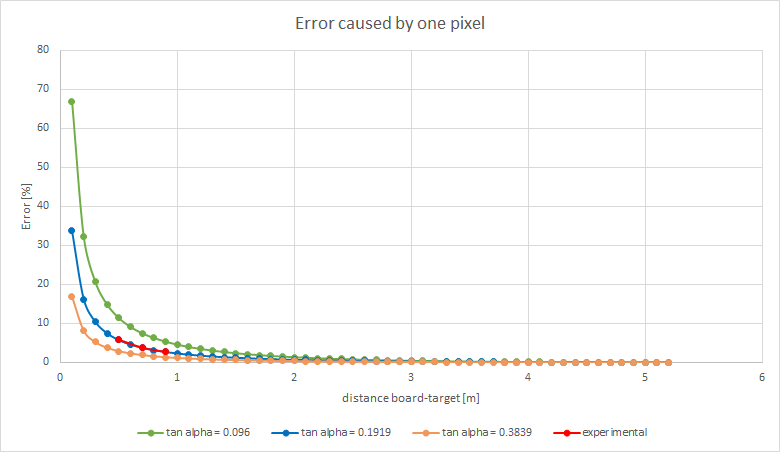
\includegraphics[scale=0.7]{fig/error.png}}
  \caption{error on the distance board-target caused by one pixel}
  \label{fig:error}
\end{figure}



\subsection{Limits of the Experiment}
The first limit of this experiment is that some pattern disorders are not taken into account. The permutation of dots that can happen with an object to far from the board has been prevented with a maximum distance board-object = 90 cm. With a greater distance than one meter, a permutation appears between the dots on the object and the ones at the left of the object but this permutation is not managed, corrected by the \emph{sort} function. Another disorder not tested is the merger of two dots. As the projector was on the ceiling, projecting slightly downward, the dots shifted horizontally but also vertically and as a consequence, the dots on the object were to high to merge with the dots on the board. Even if this kind of disorder was tested during the integration tests \ref{centroiding}, it would have been interesting to test it during the experiment.
A second limit is that, as this experiment does not include several aspects of the system designed (projector instead of the artificial light source, line of dots instead of a grid, ...), it cannot be considered as a test of this last one. Nevertheless, it permits to test the accuracy and the robustness of the algorithm tested. It is only an integration test.






\section{Outdoor Integration Testing}
\begin{figure}[!h] 
\centering
\subfigure[With Mac FaceTime HD Camera]{
  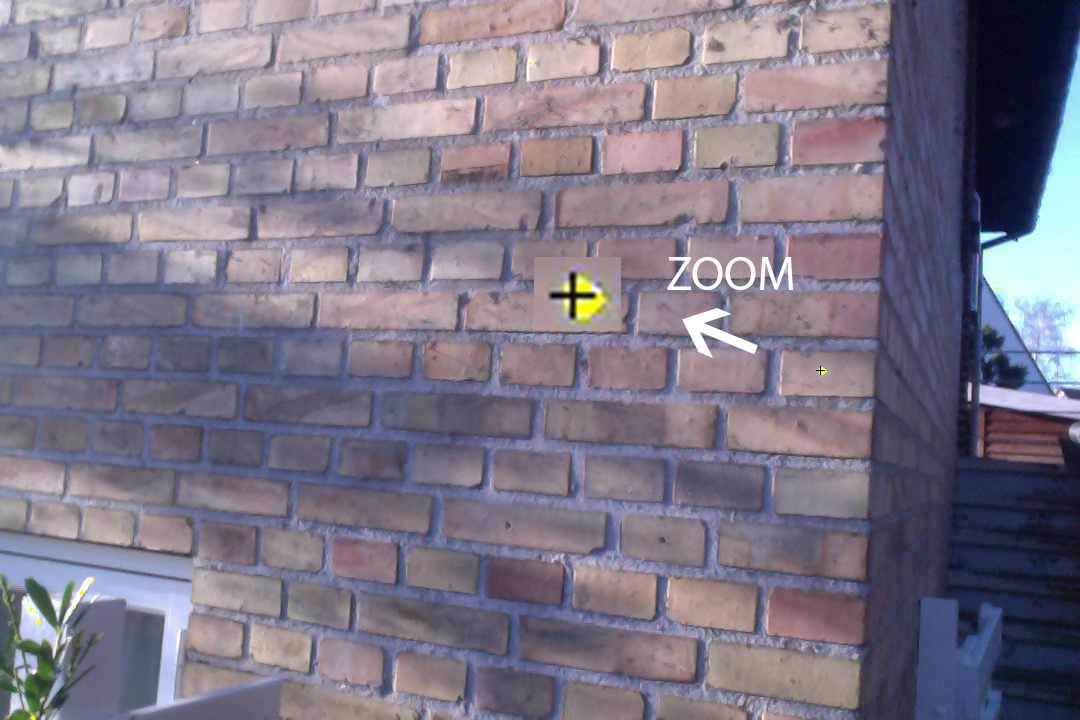
\includegraphics[scale=0.18]{fig/CentroidFrameOutdoor.png}
  \label{fig:outdoor}
}
\quad 
\quad 
\subfigure[With the Webcam Philips]{
  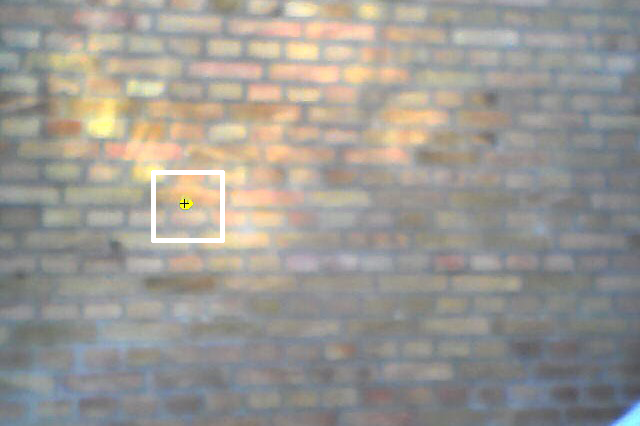
\includegraphics[scale=0.3]{fig/CentroidFrameOutdoorBlurred.png}
  \label{fig:outdoorBlurred}
}
\caption{Images Acquired by the Two Different Cameras Outdoor With Sunlight} 
\end{figure}

The two first experiments were carried out indoor. Thus, the sunlight was not taken into account, which is quite problematic since it could make impossible the color detection as the green beam will be as bright as the sun rays on the surface. In order to check if despite the sunlight, the color detection algorithm would be capable of detecting the laser beam spot on Mars, it is experimented on Earth since the sun has similar features. As the webcam used during the experiment blurs the image, another picture is acquired to make sure that it works in the two cases. The images of the test, taken around 11 am during a sunny day, are shown on figures \ref{fig:outdoor} and \ref{fig:outdoorBlurred}.

The experiment is quite conclusive. The HSV parameters were tuned and it was difficult since the spots are small and could be mistaken as noise. However, it was feasible, as it can be noticed on the figures, where the centroid is displayed in black. It is on the point even if in the first image, it is not in the center of mass because the size of the point was reduced by decreasing the noise. Since the Signal Noise Ratio on Earth with the Sunlight as noise should be similar to the one on Mars, it can be deduced that the detection of the artificial light beam spots is achievable.

%conclusion
\section*{Conclusion}
\addcontentsline{toc}{part}{Conclusion}

We designed a system permitting the 3D analysis of a martian rock using structured light and triangulation theory, and started the implementation.

Regarding the camera features, the system permits to work on a target between one and two meters far from the rover as expected. Moreover, the depth of field is also met as it is 66.5 cm and the target has a relief of 50 cm maximum. The camera features could even be changed in order to reduce a bit the depth of field and increase other properties, as instance the distance camera-target. Indeed, even if this condition is met, a bigger distance would permit an easier positioning of the rover. Also, even if the camera has not been tested, the properties comparison with the Navcam and Pancam suggests that it is well designed.

Regarding the artificial light source, it has not been tested either but the high Signal/Noise ratio indicates that the lighting points of the grid projected on the target will be bright enough to outshine the natural light and permit to have good images and a well working structured light algorithm.

Then, even if the results of the experiment with the line of dots show that the algorithm is robust but would not be rigorous enough to obtain a precise 3D map of the target, it give us good prospects. Indeed, the poor calibration suggests that the algorithm could be much more precise with an accurate calibration done with adapted tools which we did not have. The results could also be better improving the the points detection algorithm.

As regards the real time, as the system has to rectify the position of the rover's arm in order to keep the camera in focus on the target, the algorithm needs to be fast enough to send as quickly as possible the data needed for the revision of the position. This goal is also met as the algorithm using the line of dots works in real time and permits to receive the different distances continuously. (CA VA PAS, IL FAUDRAIT MEUSURER LE TEMPS !!!)\\


reste � parler de la calib matlab et des autres experiences




%futurWork
\chapter*{Future Work}
\addcontentsline{toc}{part}{Future Work}

Although the theory section and the implementation of algorithms give a solid basis to achieve the goal of the system and the experiments are promising, there is still work to do.

The first step would be carrying out the different experiments once again but with adapted tools in order to obtain a precise calibration. Moreover, the color detection algorithm could be improved in order to detect the same pixels over time. Once these two improvements done, it would be interesting to compute the new errors of the experiments to check whether or not they decrease a lot as expected and if these errors are small enough to achieve an accurate determination of the distance board-target. It would also be appreciable to carry out integration tests with the conceived artificial light source and the camera. Indeed, even if the Signal/Noise ratio calculated validates their design, tests have to be performed. For instance, it could permit to verify the depth of field, the SNR and if the camera works well with a target between one and two meters. It could also allow to implement an algorithm to adjust the shutter time linked with the luminosity of the scene over time. Then, as the algorithms work with a line of lighting dots, it should also be efficient with a grid, and thus an experiment should be executed. Finally, an integration test should be carried out on the whole system, that is to say the camera, the artificial light source plus the algorithms.

Moreover, the use of patterns could be considered instead of a grid of dots. Indeed, the projection of a pattern could permit a more detailed 3D map. We could also manipulate a grid with more points into the same surface but a lot of pattern disorders would appear into the projected grid whereas patterns such as the ones described in the Theory Section permit to detect and correct these disorders.

Also, even if the system works well, we have to be sure that it will still be the case on Mars. To do so, it would be interesting to effectuate some researches on the resistance of the components. Indeed, as we said into the section \ref{climate}, there are extreme variations in temperatures, large storms, wind and dust. Thus, the climate and the dust can damage the components or decrease their performance or even lead to malfunctions. For instance the lens of the camera striped by the dust would cause an erroneous detection of the lighting dots. Moreover, the calibration (namely the angles between the focal axis of the camera and the beams of the artificial light source) will probably change because of the vibrations during the take-off and landing of the spacecraft. Thus, a method to allow the rover to calibrate the system itself should be studied.

Once the determination of the distances camera-target will give precise results, two algorithms will need to be implemented. The first one will compute the translations and rotations between two successive 3D maps and the second one will use these results to find the parameters needed to stabilize the camera of the rover.

Finally, we need to embed the system. The mechanical and electronic issues will need to be solved. For example, the different algorithms must be embedded on processor(s). In order to choose the CPU, the issues of the computation power (the processor needs to be powerful enough to have quick run time to work in real time) and the power consumption (there is a limited power available) will need to be balanced to find an efficient compromise. Also, as the artificial light source will probably not be on board at the same level as the camera, different distances \emph{d} will have to be measured during the calibration. Indeed, as the artificial light source will probably be behind the camera, the distances \emph{d} must be measured between the camera and each beam of the light source.

\appendix
\chapter*{Appendices}
\addcontentsline{toc}{part}{Appendices}
%tableau resultat exp grid
\section{Results of the Experiment With a Line of Dots}
\label{resultsApp}
\begin{table}[H]
\centering
\caption{Object in front of dot 9 with distance object-board = 0.50 m (without noise)}
\label{res50cm}
\renewcommand{\arraystretch}{1.5}
\begin{tabular}{|c|c|c|c|c|c|}
\hline
i & $z_i$ [m] & $z_i$ error\footnotemark[1] [\%] & distance board-Object [m] & distance board-object error\footnotemark[1] [\%] \\
\hline
1 & 5.16205 & 0.92 & 0.048 & \\
\hline
2 & 5.18899 & 0.40 & 0.021 & \\
\hline
3 & 5.20282 & 0.14 & 0.007 & \\
\hline
4 & 5.20879 & 0.02 & 0.001 & \\
\hline
5 & 5.20999 & 0.00 & 0.000 & \\
\hline
6 & 5.17524 & 0.67 & 0.035 & \\
\hline 
7 & 5.21324 & 0.06 & -0.003 & \\
\hline
8 & 5.22243 & 0.24 & -0.012 & \\
\hline
9 & 4.75529 & 0.01 & 0.455 & 9.06 \\
\hline
10 & 5.27336 & 1.22 & -0.063 & \\
\hline
\end{tabular}
\end{table}
\footnotetext[1]{$error = \frac{distance_{theory}-distance_{experiment}}{distance_{theory}}100$}

\begin{table}[H]
\centering
\caption{Object in front of dots 1 and 2 with distance object-board = 0.90 m (without noise)}
\label{res90cm}
\renewcommand{\arraystretch}{1.5}
\begin{tabular}{|c|c|c|c|c|c|}
\hline
i & $z_i$ [m] & $z_i$ error [\%] & distance board-Object [m] & distance board-object error [\%] \\
\hline
1 & 4.34553 & 0.82 & 0.864 & 3.95 \\
\hline
2 & 4.36417  & 1.26 & 0.846 & 6.02 \\
\hline
3 & 5.23825 & 0.54 & -0.028 & \\
\hline
4 & 5.2443 & 0.66 & -0.034 & \\
\hline
5 & 5.20999 &	0.00 & 0.000 & \\
\hline
6 & 5.17524 &	0,67 & 0,035 & \\
\hline
7 & 5.21324	& 0,06 & -0,003 & \\
\hline
8 & 5.22243	& 0,24 & -0,012 & \\
\hline
9 & 5.27727	& 1,29 & -0,067 & \\
\hline
10 & 5.23746 & 0,53 &	-0,027 & \\
\hline
\end{tabular}
\end{table}


\begin{table}[H]
\centering
\caption{Object in front of dots 6 and 7 with distance object-board = 0.70 m and noise}
\label{res70cm}
\renewcommand{\arraystretch}{1.5}
\begin{tabular}{|c|c|c|c|c|c|}
\hline
i & $z_i$ [m] & $z_i$ error [\%] & distance board-Object [m] & distance board-object error [\%] \\
\hline
1 & 5.16204 & 0.92 & 0.048 & \\
\hline
2 & 5.18898 & 0.40 & 0.021 & \\
\hline
3 & 5.20312 & 0.13 & 0.007 & \\
\hline
4 & 5.20879 & 0.02 & 0.001 & \\
\hline
5 & 5.20999 & 0.00 & 0.000 & \\
\hline
6 & 4.53458 & 0.55 & 0.675 & 3.51 \\
\hline
7 & 4.51034 & 0.01 & 0.700 & 0.04 \\
\hline
8 & 5.22242 & 0.24 & -0.012 & \\
\hline
9 & 5.24131 & 0.60 & -0.031 & \\
\hline
10 & 5.30848 & 1.89 & -0.09848 & \\
\hline
\end{tabular}
\end{table}

\newpage
\section{LED Properties}
\label{LEDdatasheet}
\begin{figure}[h]
  %\centering
  \centerline{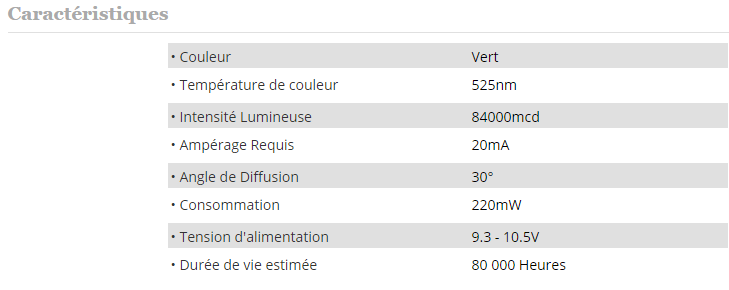
\includegraphics[scale=0.8]{fig/LedDataSheet.png}}
  \caption{LED Datasheet}
  \label{fig:LEDdatasheet}
\end{figure}

\newpage
\section{Matlab Camera Calibrator Toolbox}
\label{Toolbox}
\begin{figure}[H]
  \centering
  \centerline{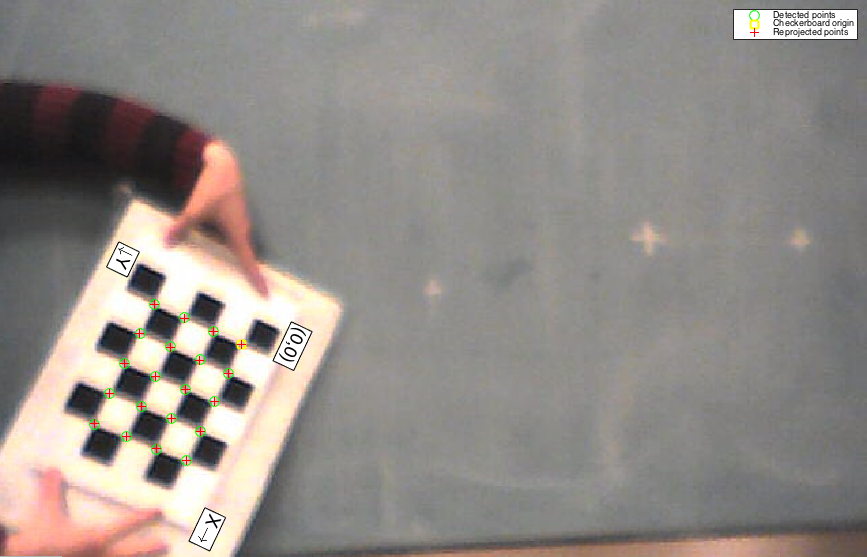
\includegraphics[scale=0.25]{fig/Checkboard.png}}
  \caption{Detection of the Checkerboard}
  \label{fig:checkerboard}
\end{figure}
\begin{figure}[H]
  \centering
  \centerline{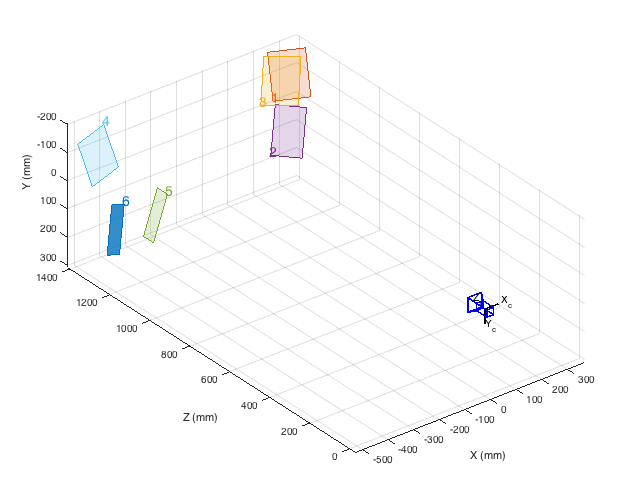
\includegraphics[scale=0.45]{fig/Extrinsics.png}}
  \caption{Distance between the different positions of the checkerboard and the camera}
  \label{fig:extrinsics}
\end{figure}

\newpage
\section{CCD Properties}
\label{CCDdatasheet}
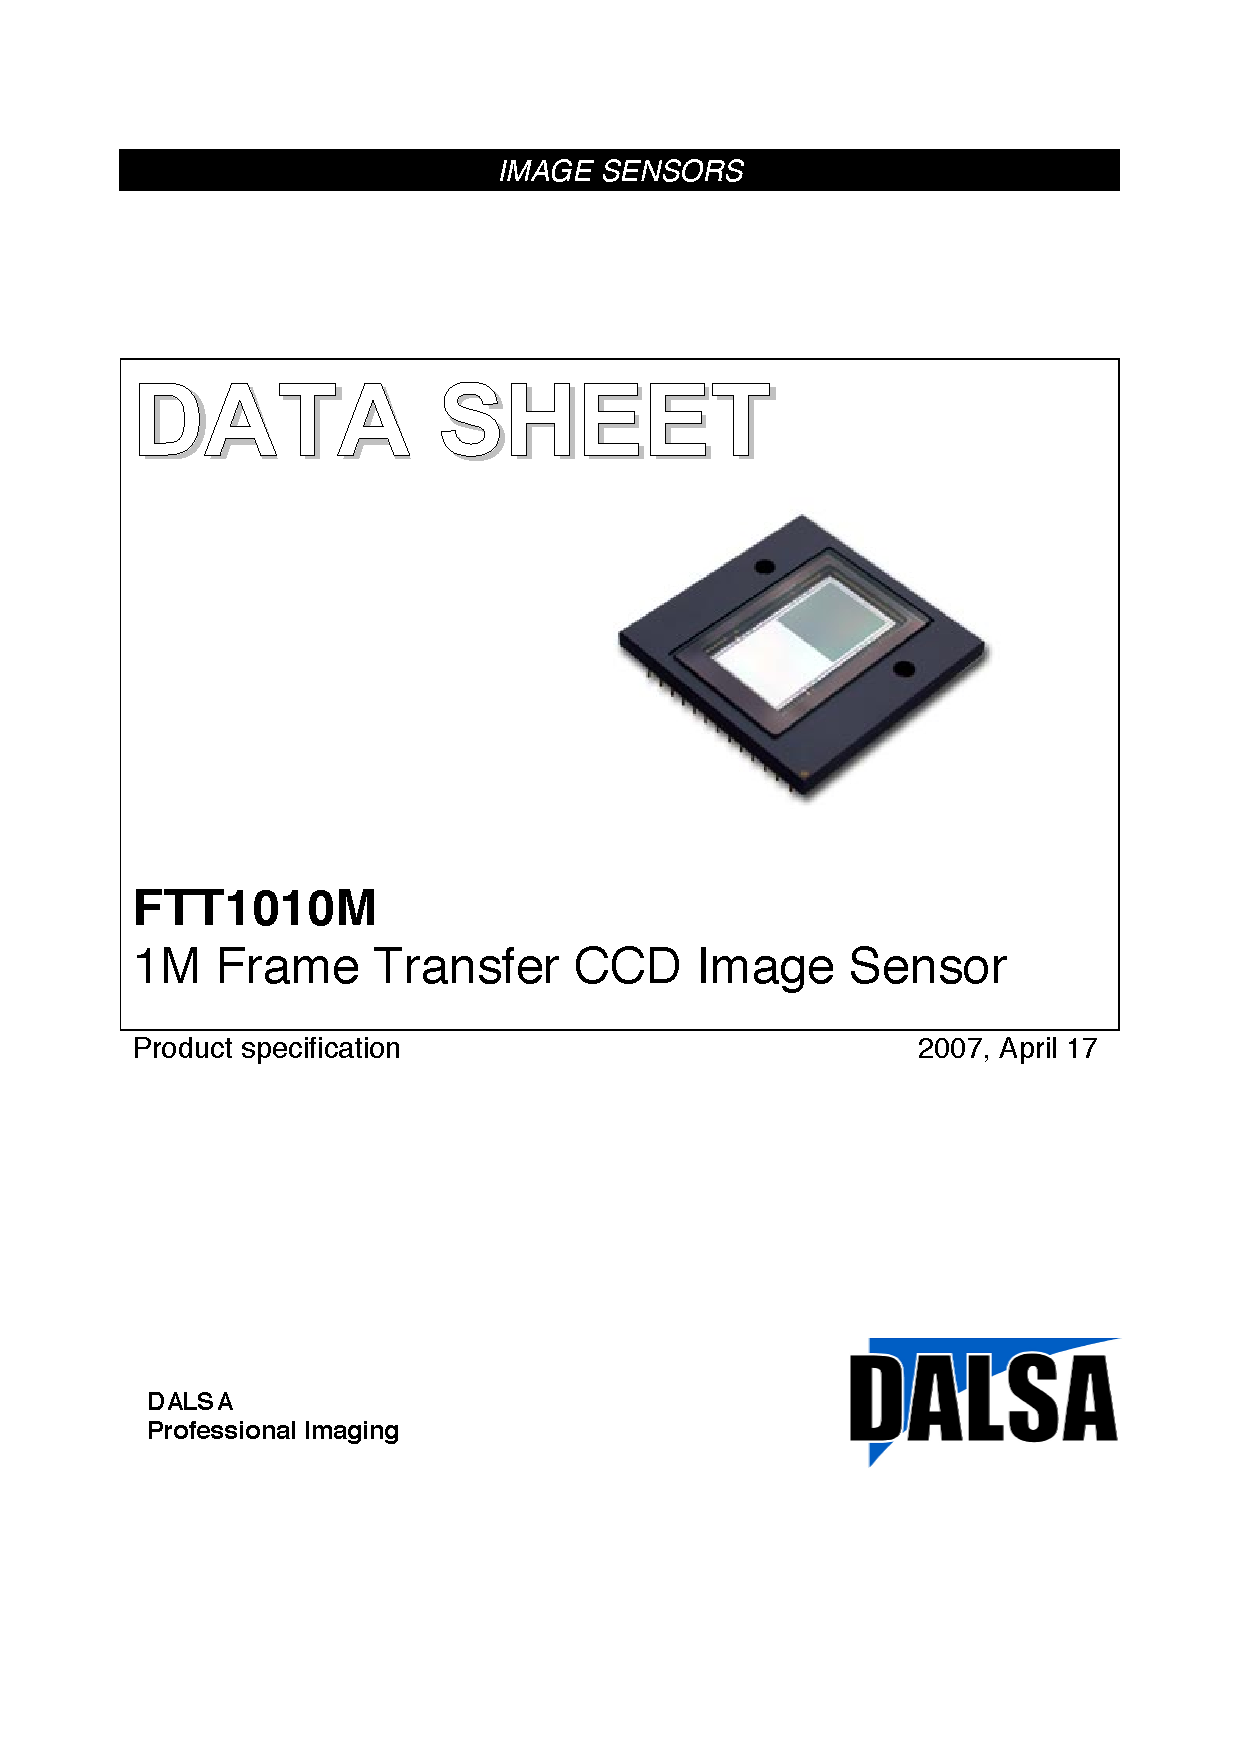
\includepdf[pages = {1-18}]{fig/CCDdatasheet.pdf}

%\end{appendices}

\bibliography{bibliographie}
\addcontentsline{toc}{part}{Bibliography}
\bibliographystyle{plain}

\end{document}
